% \documentclass{ieeeaccess}
\documentclass[journal]{IEEEtran} 
%Adjusted 05/13/2026 at the byline author names
\usepackage{caption}
\usepackage{xurl}
\usepackage{cite}
\usepackage{amsmath,amssymb,amsfonts}

\usepackage{graphicx}
\usepackage{enumitem}
\usepackage{subcaption}
\usepackage{amsthm}
\usepackage{textcomp}
\usepackage{algorithm}
\usepackage{algpseudocode}  
\usepackage{float}
\usepackage{xspace}
\usepackage[table]{xcolor}
\usepackage{booktabs}
% \usepackage{svg}
\definecolor{codehl}{RGB}{255,245,200}

\usepackage{bm}
\makeatletter
\AtBeginDocument{\DeclareMathVersion{bold}
\DeclareSymbolFont{NewLetters}{T1}{times}{b}{it}
\SetSymbolFont{operators}{bold}{T1}{times}{b}{n}
\SetSymbolFont{NewLetters}{bold}{T1}{times}{b}{it}
\SetMathAlphabet{\mathrm}{bold}{T1}{times}{b}{n}
\SetMathAlphabet{\mathit}{bold}{T1}{times}{b}{it}
\SetMathAlphabet{\mathbf}{bold}{T1}{times}{b}{n}
\SetMathAlphabet{\mathtt}{bold}{OT1}{pcr}{b}{n}
\SetSymbolFont{symbols}{bold}{OMS}{cmsy}{b}{n}
\renewcommand\boldmath{\@nomath\boldmath\mathversion{bold}}}
\makeatother

\def\BibTeX{{\rm B\kern-.05em{\sc i\kern-.025em b}\kern-.08em
    T\kern-.1667em\lower.7ex\hbox{E}\kern-.125emX}}


% Custom algorithmic keywords
\algnewcommand{\Notation}{\item[\textbf{Notation:}]}
\algnewcommand{\Output}{\item[\textbf{Output:}]}

\newcommand{\kms}{km\,s$^{-1}$}
% \newcommand{\msun}{$M_\odot}
\newcommand{\msun}{$M_\odot$}
\newcommand\oak[1]{\textcolor{red}{OAK: #1}}
\newcommand\ben[1]{\textcolor{blue}{#1}}
\newcommand\ignore[1]{}
\newcommand{\rtsmarm}{SMARM+\xspace}
\newcommand{\rtsmarmone}{SMARM+PRNG\xspace}
\newcommand{\rtsmarmtwo}{SMARM+FPE\xspace}

\newcommand{\acron}{SMARM+\xspace}
\newcommand{\smarm}{SMARM\xspace}

\newtheorem{definition}{Definition}
\newtheorem{assumption}{Assumption}[section]
\newtheorem{lemma}{Lemma}[section]
\newtheorem{theorem}{Theorem}[section]
\newtheorem{corollary}{Corollary}[section]
\newcommand{\Adv}{\mathbf{Adv}}




%Your document starts from here ___________________________________________________
\begin{document}
%\history{Date of publication xxxx 00, 0000, date of current version xxxx 00, 0000.}
% \doi{10.1109/ACCESS.2024.0429000}

\title{SMARM+: Analyzing and Enhancing Shuffled Measurements for Remote Attestation in Real-Time IoT Settings}
\author{
\IEEEauthorblockN{Amarin Laohajirapan}
\IEEEauthorblockA{\textit{College of Computing,} Prince of Songkla University, Phuket Campus, Thailand\\
Email: 6730621007@psu.ac.th}
\and
\IEEEauthorblockN{Norrathep Rattanavipanon\thanks{Corresponding author: norrathep.r@psu.ac.th}}
\IEEEauthorblockA{\textit{College of Computing,} Prince of Songkla University, Phuket Campus, Thailand\\
Email: norrathep.r@psu.ac.th}
}

\maketitle


\begin{abstract}
Remote attestation (RA) is a lightweight security primitive for detecting software compromise on IoT devices. Traditional RA schemes require atomic, non-interruptible memory measurements, making them difficult to deploy alongside real-time workloads. SMARM addresses this limitation by measuring memory in a secret, shuffled block order, reducing the non-interruptibility period to the duration of a single block measurement. However, SMARM was originally designed for microkernel-based systems and has not been studied in RTOS-driven real-time environments.


% In this work, we present the first systematic study of SMARM in real-time RTOS-based setups. We implement SMARM on commodity ARM TrustZone-M hardware running FreeRTOS and Zephyr, and introduce the \emph{Frequency Accuracy Ratio} (FAR) to quantify the extent to which attestation can coexist with real-time execution under varying workloads. Our evaluation shows that SMARM’s real-time compatibility is highly sensitive to block size: large blocks significantly degrade real-time availability, while small blocks incur substantial secure-storage overhead, limiting deployability on memory-constrained devices.

% To address this limitation, we propose SMARM+, a family of enhanced SMARM variants consisting of SMARM+PRNG and SMARM+FPE. They are designed to reduce secure-storage requirements while preserving SMARM’s security guarantees and real-time behavior. Our evaluation highlights the trade-off between secure-storage reduction, attestation runtime, and energy overhead, and provides guidance on selecting among SMARM, SMARM+PRNG, and SMARM+FPE for different deployment settings.
In this work, we present \ben{a systematic study} of SMARM in real-time RTOS-based setups. We implement SMARM on commodity ARM TrustZone-M hardware running FreeRTOS and Zephyr, and introduce the \emph{Frequency Accuracy Ratio} (FAR) to quantify the extent to which attestation can coexist with real-time execution under varying workloads. Our evaluation shows that SMARM’s \ben{interference with real-time tasks, as measured by FAR,} is highly sensitive to block size: large blocks significantly degrade real-time availability, while small blocks incur substantial secure-storage overhead, limiting deployability on memory-constrained devices.

To address this limitation, we propose SMARM+, a family of enhanced SMARM variants consisting of SMARM+PRNG and SMARM+FPE. They are designed to reduce secure-storage requirements \ben{while satisfying the same security requirements as SMARM and retaining comparable real-time behavior, as measured by FAR}. Our evaluation highlights the trade-off between secure-storage reduction, attestation runtime, and energy overhead, and provides guidance on selecting among SMARM, SMARM+PRNG, and SMARM+FPE for different deployment settings.


\end{abstract}

\begin{IEEEkeywords}
Remote attestation, real-time IoT systems, TrustZone-M, RTOS, IoT security, format-preserving encryption.
\end{IEEEkeywords}

% \titlepgskip=-21pt

\maketitle


\section{Introduction}
\label{introduction}

Internet-of-Things (IoT) devices have become integral to modern society, widely deployed in many domains, such as smart healthcare, industrial automation, and smart infrastructure.
\ben{As their deployment continues to grow, they have also become attractive targets for large-scale malware attacks, as exemplified by the Mirai botnet~\cite{antonakakis2017mirai,kolias2017mirai}.}
However, due to the resource-constrained nature, deploying sophisticated security mechanisms (e.g., anti-virus) is often impractical in IoT devices.

To address this challenge, Remote Attestation (RA) has emerged as a lightweight security primitive for detecting software compromise on such devices.
At a high level, it is a challenge-response protocol between a constrained IoT device, referred to as the \emph{prover}, and a more powerful entity acting as the \emph{verifier}.
As illustrated in Figure~\ref{fig:ra-overview}, a typical RA protocol consists of three steps:



\begin{figure}[!htp]
    \centering
    \includegraphics[width=\linewidth]{ra_overview1.pdf}
    \caption{Remote Attestation (RA) workflow and memory measurement strategies.}
    \label{fig:ra-overview}
\end{figure}

\begin{enumerate}[label={(\arabic*)}]
    \item The verifier sends a fresh challenge (e.g., a random nonce or a monotonically increasing counter) to the prover.
    \item Upon receiving the challenge, the prover computes an authenticated integrity measurement -- realized as either a message authentication code (MAC) or a digital signature -- over its program memory along with the received challenge, and returns the result as attestation evidence to the verifier.
    \item The verifier checks the evidence against a reference value for the expected memory contents.
\end{enumerate}


To prevent \emph{roving} malware~\cite{smarm} that relocates itself to evade detection, traditional RA techniques~\cite{smart,hydra,vrased} require the computation in Step (2) to execute atomically, i.e., with interrupts disabled.
While effective, this approach also prevents normal applications from executing in Step (2), rendering such schemes unsuitable for real-time systems.

SMARM~\cite{smarm} was proposed as an alternative memory measurement strategy to relax the atomicity requirement.
As illustrated in Figure~\ref{fig:ra-overview}, rather than measuring program memory sequentially with interrupts disabled, SMARM allows interrupts to be re-enabled after each memory block is measured.
On its own, this relaxation would permit roving malware to interrupt the measurement task in Step (2) and relocate itself to evade detection.
Hence, SMARM proposes an additional technique to mitigate this by measuring the memory blocks in a \emph{private} and \emph{random} (i.e., shuffled) order.
To be secure, SMARM safeguards the shuffled order in a secure storage that cannot be accessed by untrusted software.
Intuitively, since the roving malware does not know which memory blocks have already been measured, its probability of successfully evading detection is significantly reduced.
With this technique, SMARM reduces the non-interruptibility period from the entire program memory to a single-block measurement.

In this work, we observe two limitations of SMARM.
First, SMARM was designed and prototyped atop the HYDRA architecture~\cite{hydra}, which relies on a formally verified seL4 microkernel~\cite{sel4} to secure the measurement task and store the shuffled order.
While this design provides strong security guarantees due to the formal verification of seL4, real-time IoT deployments commonly rely on lightweight RTOSes such as FreeRTOS, rather than microkernel-based systems.
As such, it limits the practicality and wide-scale adoption of SMARM in RTOS-based systems.
Second, SMARM was evaluated in experimental settings that do not consider real-time workloads.
Although the results show a significant reduction in the non-interruptibility period, it remains unclear whether SMARM can truly co-exist with real-time systems.

In light of these limitations, this work makes the following contributions:

\begin{itemize}\sloppy
    \item \textbf{Design and implementation of SMARM on RTOS-based platforms (Section~\ref{sec:porting}).}
    We present a design and implementation of SMARM that is compatible with widely-adopted RTOSes.
     The key challenge is to \ben{satisfy SMARM's security requirements (S1)--(S3)} without relying on a formally verified microkernel, while maintaining compatibility with RTOS-based execution environments.
    To resolve this challenge, our design leverages the ARM TrustZone-M security extension as a trust anchor in place of seL4.
    \ben{TrustZone-M is part of the Armv8-M architecture~\cite{armv8m-arm} and is available on commercial off-the-shelf microcontrollers~\cite{tzm-sec-iot,stm32l552_nucleo144}}.
    
    \item \textbf{Evaluation of SMARM under real-time workloads (Section~\ref{sec:evaluation}).}
    Our primary FreeRTOS evaluation establishes the trade-off between real-time coexistence and secure storage.
    To quantify task execution frequency during attestation, we introduce a new metric, \emph{Frequency Accuracy Ratio (FAR)}, which measures task execution frequency relative to the baseline.
    Our results show that SMARM's \ben{interference with real-time tasks} is highly sensitive to the measurement block size: small blocks preserve near-nominal task execution frequency \ben{as measured by FAR}, whereas FAR decreases at larger block sizes in the tested FreeRTOS configuration.
    Smaller blocks shorten the non-interruptibility period and increase the storage required for the permutation, exposing a key limitation for deployment on highly resource-constrained MCUs.
    A supporting Zephyr/TF-M evaluation examines whether the block-size-related interference observed in the primary FreeRTOS evaluation also occurs with a different RTOS and Secure-world runtime.
 
 
    \item \textbf{Reducing SMARM's permutation-state storage (Section~\ref{sec:resmarm-design}-\ref{sec:rtsmarm-evaluation}).}
    We propose \acron, enhanced variants of SMARM that reduce secure-storage requirements.
    Under the assumptions of our security analysis, both variants satisfy SMARM's security requirements (S1)--(S3).
    The first variant (\rtsmarmone) reduces permutation-state storage from $O(n \log n)$ to $O(n)$ bits while the second (\rtsmarmtwo) further reduces \ben{permutation-state storage to $O(1)$, independent of $n$}.
    Our FreeRTOS evaluation shows FAR comparable to SMARM at the same block size, together with a trade-off among measured Secure-memory footprint, end-to-end attestation runtime, and board-level energy consumption.
    %At the recommended operating point ($B = 1024$~bytes), \rtsmarmone incurs only $5\%$ energy overhead over SMARM baseline, while \rtsmarmtwo incurs $52\%$, reflecting its constant per-block cryptographic cost.

\end{itemize}


\section{Background}\label{sec:background}
This section reviews the background of SMARM and ARM TrustZone-M architecture used as basis in this work.
%and two representative RTOSs: FreeRTOS and Zephyr.

\subsection{SMARM: Shuffled Measurements Against Roving Malware}\label{subsec:smarm}

Remote attestation (RA) for low-end embedded devices has traditionally
relied on \emph{atomic} memory measurements, as in SMART, HYDRA,
and VRASED, where the entire attested memory region is hashed in a
single non-interruptible sweep with interrupts disabled~\cite{smart,hydra,vrased,ra_survey}. These designs provide strong security guarantees but inherently conflict with real-time workloads, since they block all interrupts for a period that scales with the size of the attested memory.
The key idea of SMARM~\cite{smarm} is to enhance the RA workflow (see Figure~\ref{fig:ra-overview}) by measuring memory in a shuffled (i.e., unpredictable and private) order. Specifically, SMARM partitions the prover's memory into $n$ fixed-size blocks,
$M = \{M_1, \ldots, M_n\}$, which are measured according to a one-time shuffled order rather than a fixed/predictable sequence.

Figure~\ref{fig:smarm_state} illustrates the SMARM workflow.
Upon receiving a one-time challenge, $chal$, from the verifier, a secure environment on the prover computes an attestation response via the following steps:


\begin{figure}[!htp]
    \centering
    \includegraphics[width=\linewidth]{state-diagram}
    \caption{The workflow of SMARM~\cite{smarm}}
    \label{fig:smarm_state}
\end{figure}

\begin{enumerate}
    \item \textbf{Permutation Generation.}
    The prover computes a permutation $\sigma$ over the memory block indices $[1,\ldots,n]$, where $\sigma$ determines the measurement order for the current attestation instance, i.e., the block $M_{\sigma(i)}$ is measured at step $i$.
    SMARM's main security requires $\sigma$ to be \emph{fresh} and \emph{private} for each attestation instance;
    to achieve these, SMARM instantiates this permutation using the Fisher-Yates shuffle method~\cite{fisherYates}:
    \[
        \sigma = \mathsf{FisherYates}(seed, [0,\ldots,n-1]),
    \]
    where its PRNG $seed$ is derived from $k$ and $chal$: $k$ is a pre-shared secret key between the prover and the verifier, and $chal$ is the verifier’s challenge.
    After this, it stores $\sigma$ in secure storage and initializes the loop counter $i$ to $0$.

    \item \textbf{Atomic Block Measurement.}
    At iteration $i$, the prover's secure environment retrieves $\sigma(i)$ from secure storage, disables system-wide interrupts, and measures (i.e., hashes) the corresponding memory block $M_{\sigma(i)}$.
    After the measurement, it re-enables interrupts and increments $i$.

    \item \textbf{Loop Check.}
    The secure environment checks whether all memory blocks have been measured by testing whether $i = n$.
    If not, it repeats the previous step.

    \item \textbf{Finalization.}
    After all blocks in $M$ have been measured, the prover's secure environment computes a MAC over the final measurement using the key $k$ and sends the result to the verifier as the attestation response.
    With possession of $k$ and $chal$, the verifier can reconstruct the permutation used in the current instance and thereby validate the received attestation response against the expected measurement of~$M$. \ben{In SMARM, freshness is enforced by \emph{order-based challenge binding}: $chal$ determines $\sigma$ and thus the concatenation order over which the MAC is accumulated, so a stale or substituted challenge yields a different order and fails verification (except with negligible probability).
    Our realization additionally authenticates $chal$ explicitly, together with the attestation parameters (Section~\ref{sec:porting}).}

\end{enumerate}

\paragraph{\textbf{Security}}
SMARM considers a threat model in which the adversary can exploit software vulnerabilities on the prover to gain control over all software except for the secure execution environment and secure storage.
In particular, the adversary is allowed to read/write and execute arbitrary code anywhere in the prover's memory.
In addition, SMARM assumes a \emph{Knowledge of Future Volume} (KFV) malware, which may use the aforementioned capabilities to interrupt the secure execution after each block measurement and learn \emph{how many} memory blocks have already been measured.

Under this threat model, SMARM provides a theoretical analysis of its defense.
Assuming the worst-case scenario in which the malware fits entirely within a single memory block, the optimal evasion strategy for KFV malware is to interrupt after each block measurement and relocate itself to a different block.
For large $n$, this strategy yields an evasion probability converged
to approximately $37\%$~\cite{smarm}.
To increase the likelihood of detection, SMARM proposes repeating
the shuffled measurements multiple times for each attestation instance;
for example, performing the shuffled measurements seven times reduces
the evasion probability to below $10^{-3}$~\cite{smarm}.

To meet security, SMARM assumes architectural support for a secure execution environment that provides the following security guarantees:
\begin{itemize}
    \item[(S1)] \emph{Controlled execution:} the attestation code can only be invoked and return via well-defined entry and exit points (i.e., no mid-code entry or early exit), and it may only be interrupted between consecutive block measurements;
    \item[(S2)] \emph{Key secrecy:} the attestation key~$k$ is accessible exclusively to the attestation code; and
    \item[(S3)] \emph{Private measurement order:} the order in which memory blocks are measured must not be known by KFV malware. This is realized by keeping the permutation~$\sigma$ in memory that is inaccessible to untrusted software.
\end{itemize}


\begin{figure}[!htp]
    \centering
    \includegraphics[width=\linewidth]{hydra-smarm.png}
    \caption{SMARM prototype atop the HYDRA architecture.}
    \label{fig:hydra_impl}
\end{figure}



\paragraph{\textbf{Implementation}}
In its prototype (shown in Figure~\ref{fig:hydra_impl}), SMARM realizes this secure execution environment using the HYDRA architecture~\cite{hydra}, which targets MMU-equipped devices and is built atop the formally verified seL4 microkernel~\cite{sel4}.
Leveraging seL4's verified isolation properties, HYDRA executes the attestation code within a privileged user-space task, referred to as the \emph{measurement task}.
This task is isolated from all other user-space tasks, can access all device memory required for measurement while its own memory remains inaccessible to other tasks.

To enforce (S1), the measurement task can only be invoked via a dedicated IPC endpoint and returns solely with the attestation response.
At runtime, the measurement task is initially assigned the highest priority, ensuring that it cannot be preempted while measuring a memory block.
After completing each block measurement, the task lowers its priority and explicitly yields the CPU execution, allowing other tasks (malicious or real-time tasks) to execute between consecutive measurements.
When the measurement task is scheduled again, it restores its priority to the highest level and proceeds with the next atomic block measurement.
%
Finally, HYDRA configures access control of memory regions in seL4 such that only the measurement task can access $k$ and $\sigma$, thereby satisfying (S2) and (S3).

\paragraph{\textbf{Evaluation}}
The security of SMARM fundamentally relies on the secrecy of the permutation~$\sigma$, which necessitates secure storage that is inaccessible to untrusted software.
For a prover memory $M$ partitioned into $n$ blocks, SMARM requires at least
$|\sigma| = n \cdot \lceil \log_2 n \rceil$ bits of secure storage to store $\sigma$, making the overhead linear in~$n$.

Reducing the secure storage requirement therefore necessitates lowering the value of $n$.
However, as each block has size $B = |M|/n$, a smaller $n$ implies a larger block size to be measured atomically.
This, in turn, increases the non-interruptibility period $t_{\text{disabled}}$ during attestation in SMARM.

As a result, SMARM exhibits an inherent trade-off between secure storage size and real-time availability.
SMARM evaluates this trade-off on the i.MX6 SabreLite platform, a development board representative of low-cost IoT devices\cite{smarm,sabreLite}.
Figure~\ref{fig:smarm_tdisabled} illustrates the tension: increasing the block size $B$ (equivalent to reducing $n$) alleviates the secure storage requirement, but it also increases $t_{\text{disabled}}$.
Conversely, selecting a small $B$ minimizes $t_{\text{disabled}}$ (improving real-time availability during attestation) at the cost of a much larger secure storage overhead, which may be impractical for resource-constrained devices.


\begin{figure}[!h]
    \centering
    \includegraphics[width=\linewidth]{smarm_tdisabled.pdf}
    \caption{SMARM trade-off between non-interruptibility period $t_{\text{disabled}}$
    and secure storage requirement $|\sigma|$
    for a fixed memory size $|M| = 256\,\text{MB}$ on the i.MX6 SabreLite device.}
    \label{fig:smarm_tdisabled}
\end{figure}

In addition, SMARM performed an additional experiment that evaluates the overall attestation runtime under different values of two parameters: $t_{\text{disabled}}$ and $t_{\text{slice}}$, where the latter represents a time-slice duration that a normal application task runs between consecutive block measurements.
The results showed that both $t_{\text{disabled}}$ and $t_{\text{slice}}$ directly affect the total attestation time with their high value leading to a longer attestation time.
Nonetheless, the work in~\cite{smarm} \emph{did not} evaluate the extent to which the SMARM technique impacts the real-time guarantees of time-sensitive tasks, leaving it unclear which block size should be used in a given strict real-time setting.

\subsection{TrustZone-M Architecture}\label{subsec:tzm}



ARM TrustZone for Cortex-M~\cite{arm-trustzone-cm} (or TrustZone-M in short) provides a production-ready Trusted Execution Environment (TEE) for low-cost IoT devices.
\ben{TrustZone-M is the optional security extension of the Armv8-M architecture~\cite{armv8m-arm} and is available on commercial Cortex-M23/M33-based microcontrollers, including the STM32L552 used in this work~\cite{tzm-sec-iot,stm32l552_nucleo144}.}
It provides hardware-enforced isolation by partitioning software execution into two isolated runtime environments: the \emph{Secure} and \emph{Non-Secure} worlds.

Following the TEE's design principle, TrustZone-M runs untrusted application software (including RTOS and user applications) in the Non-Secure world, while placing small security-critical software in the Secure world.
Although isolated, both worlds still execute on the same physical CPU core, sharing the system's interrupts;
these interrupts are globally managed by the Nested Vectored Interrupt Controller (NVIC), allowing interrupts to happen cross-world boundaries.
As a result, execution in the Secure world may be interrupted by the Non-Secure world; also it is possible for the Secure world to disable all sources of interrupts (e.g., via the \texttt{CPSID} instruction), thereby preventing the Non-Secure world from executing and enabling atomic execution of a Secure-world function.

In this work, we rely on the following security properties offered by TrustZone-M:

\begin{itemize}
    \item \textbf{Isolation at Hardware Level.}
    TrustZone-M provides strong separation between the Secure and Non-Secure worlds through dedicated hardware components: the Security Attribution Unit (SAU) and the Implementation-Defined Attribution Unit (IDAU), which jointly define the security attribution of memory and peripherals at the hardware level~\cite{arm-trustzone-cm}.
    These components govern access to all system resources including program/data memory and peripherals.
    As a result, code executing in the Non-Secure world cannot read or modify Secure-world code or data, even in the presence of a fully compromised Non-Secure software stack.

    \item \textbf{Restricted Secure-World Entry.}
    TrustZone-M restricts access to Secure-world functionality to a set of explicitly defined entry points located in the \emph{Non-Secure Callable} (NSC) region.
    This region is part of Secure memory and is protected from modification by Non-Secure software.
    Together with TrustZone-M's secure state transition mechanism (enforced in hardware), this restriction ensures that Secure-world functions are invoked only in their entirety.
\end{itemize}


\ben{A recent security study of TrustZone-M-based IoT systems shows that misconfiguration and improper partitioning of memory and peripherals can undermine the intended isolation guarantees, leading to practical exploits even when the hardware security extensions are present~\cite{tzm-sec-iot}.}
These findings motivate our use of TrustZone-M as a tightly scoped root of trust: \rtsmarm confines security-critical state (e.g., attestation keys and permutation
metadata) to the Secure world, while treating the Non-Secure RTOS and application stack as fully adversarial.

\section{Realization of SMARM on RTOS-based Systems}
\label{sec:porting}

This section describes our efforts to realize SMARM in RTOS systems.
We begin by discussing the non-trivial challenges that preclude a simple extension of existing SMARM prototype (HYDRA-based one) to RTOS, thereby motivating the need for a new direction in this work.




\subsection{Challenges of Adapting SMARM to RTOS}\label{subsec:naive}

A naive approach is to adapt HYDRA-based prototype of SMARM to operate atop an RTOS.
In principle, this would correspond to replacing the seL4 microkernel with an RTOS kernel while leaving user-level tasks (including the measurement task) unchanged.
However, such an approach raises several security issues.


Recall the HYDRA-based SMARM prototype in Figure~\ref{fig:hydra_impl}.
First, to satisfy (S1)-(S3), it relies on seL4's isolation guarantees to protect the measurement task (that implements the SMARM logic) from other untrusted tasks.
These isolation guarantees are absent in commonly deployed RTOSes.
For example, vanilla FreeRTOS~\cite{freertos}, the most commonly used RTOS in commercial real-time embedded systems, operates under bare-metal settings in which all tasks execute at the same privilege level.
As a result, other (potentially compromised) tasks can freely access all system resources, including $k$ and $\sigma$ used by the measurement task, hence easily breaking (S2) and (S3).
Similarly, the default configuration of NuttX~\cite{nuttx} provides no inter-task isolation.

Even when considering RTOSes that offer some form of memory isolation, e.g., the MPU version of FreeRTOS~\cite{freertos-mpu} or Zephyr OS~\cite{zephyr}, these protections are not backed by formal verification, unlike seL4.
This means their security guarantees only hold as long as the kernel itself remains uncompromised.
In practice, these RTOSes have been shown to contain many kernel-level vulnerabilities, e.g., CVE-2018-16525 that enables remote code execution in FreeRTOS or CVE-2024-6137 that leads to malicious writes to Zephyr's kernel memory~\cite{cve_freertos_rce,cve_zephyr_memory}.
An adversary can exploit such vulnerabilities to break isolation, rendering SMARM insecure on these platforms.

Therefore, simply replacing seL4 with an RTOS of choice is insufficient to make SMARM \emph{secure}.
Instead, our design leverages ARM TrustZone-M to provide hardware-enforced isolation mechanisms available on off-the-shelf embedded platforms.
Next, we describe the system model considered in this work, followed by the corresponding threat model.


\subsection{System \& Threat Model}

\begin{figure}[!htp]
    \centering
    % ปรับขนาด width ตามความเหมาะสมของหน้ากระดาษ (แนะนำ 0.9 หรือ 1.0)
    \includegraphics[width=1.0\linewidth]{system-threat-model.pdf}
    \caption{Our proposal of SMARM on RTOS using TrustZone-M}
    \label{fig:system_threat_model}
\end{figure}


We consider a prover implemented on an ARM Cortex-M device equipped with TrustZone-M, which divides execution into two runtime environments: the Secure world (trusted TEE) and Non-Secure worlds (untrusted).
The Non-Secure world hosts untrusted software including the RTOS kernel and real-time application tasks.
In contrast, SMARM's security-critical logic is assumed to be trusted, resides in the Secure world and is accessible from the Non-Secure world only via a NSC call.

We adopt the same threat model as SMARM: an adversary can exploit software vulnerabilities to gain full control over all untrusted software.
Under our system model, this corresponds to the adversary fully compromising the entire Non-Secure world.
Since the Secure world is assumed to be trusted, the adversary cannot tamper with the SMARM logic residing in the Secure world.
%
In addition, we consider KFV malware that can interrupt Secure-world execution after each block measurement (via NVIC control; see Section~\ref{subsec:tzm}), with the aim of relocating malicious code across memory blocks to evade detection.
%
Following SMARM, we consider hardware/physical attacks, side-channel attacks and denial-of-service (DoS) attacks to be out of scope.\ben{More precisely, physical side-channel analysis, fault injection, and invasive hardware modification are orthogonal to this work and require dedicated countermeasures~\cite{kiri2026vecodi}.
Timing information that Non-Secure software can observe through interrupts and resumption, however, is within scope and is addressed in Section~\ref{sec:rtsmarm-bitarray}.
Following the typical TrustZone-M trust model~\cite{kiri2026vecodi,an5347}, we assume a secure boot process that guarantees the integrity of the Secure-world image at boot, a master key~$k$ provisioned into Secure-only flash and shared with the verifier, and a security DMA controller that prevents Non-Secure bus masters from accessing Secure memory, such as the Global TrustZone Controller (GTZC) of our STM32L552 platform.
Section~\ref{sec:platform-config} details how our realization configures and relies on these mechanisms.}




\subsection{SMARM on RTOS using TrustZone-M}

We propose a new realization of SMARM that coexists with an RTOS and real-time application tasks without requiring custom hardware.
Unlike the naive approach discussed in Section~\ref{subsec:naive}, this design leverages the hardware-enforced isolation provided by TrustZone-M, retaining SMARM's security even if an adversary fully compromises all untrusted software in the Non-Secure world.

\subsubsection{Components}

In addition to the unmodified RTOS kernel and real-time application tasks, we decompose SMARM into two components, as illustrated in Figure~\ref{fig:system_threat_model}.

\textbf{Wrapper Task.}
The Wrapper Task is implemented as a regular RTOS task executing in the Non-Secure world.
It serves as an interface between the verifier (or other tasks responsible for prover-verifier communication) and the Secure-world SMARM logic.
Upon receiving an attestation request, the wrapper task invokes the Secure Service, obtains the attestation evidence, and forwards it to the verifier.
To allow preemption by real-time tasks, we configure the wrapper task to run at the lowest priority.
    
\textbf{Secure Service.}
The Secure Service resides entirely in the Secure world and is exposed to the Non-Secure world via an NSC entry point.
When invoked with an attestation request, it executes the SMARM logic as described in Section~\ref{subsec:smarm} and detailed in Algorithm~\ref{alg:smarm_baseline}, then returning the attestation evidence to the caller.
To enforce atomic block measurements, the service disables interrupts via the \texttt{CPSID} instruction immediately before each block measurement and re-enables them upon completion.
As a result, (S1) is guaranteed in this design by preventing partial execution of the Secure Service and disallowing interruptions during block measurements.
    
To satisfy (S2), we store the master attestation key~$k$ persistently in Secure storage that is accessible only from the Secure world.
% (e.g.,~\cite{tzm-sec-iot,silabs-secure-key-storage}).
At runtime, all $k$-related materials reside in Secure RAM, which is inaccessible to the Non-Secure world.
Similarly, to satisfy (S3), the permutation~$\sigma$, once generated, is not exposed to Non-Secure RAM and therefore cannot be inferred by KFV malware.
KFV malware cannot also perform replay attacks since $\sigma$ is based on a one-time challenge $chal$ and a secret $k$.

\ben{\paragraph{Key hierarchy and domain separation.}
Following standard cryptographic engineering practice~\cite{krawczyk2010hkdf,nist-sp800-108}, we do not use the master key $k$ directly for multiple purposes.
Instead, we derive purpose-specific keys via a PRF-based KDF with distinct domain-separation labels:
\[
  k_{\mathrm{prp}} \gets \mathsf{KDF}(0 \,\|\, k),
  \qquad
  k_{\mathrm{mac}} \gets \mathsf{KDF}(1 \,\|\, k),
\]
where the labels $0$ and $1$ distinguish order-generation (permutation/PRNG/FFX) from attestation-MAC usage, and $\mathsf{KDF}(\ell \,\|\, k)$ is instantiated as $\mathsf{HMAC\text{-}SHA256}(k,\ell)$.
Algorithms~\ref{alg:smarm_baseline}--\ref{alg:rtsmarm-fpe} then use $k_{\mathrm{prp}}$ to derive the measurement order and $k_{\mathrm{mac}}$ for HMAC; both derived keys remain in Secure memory under (S2).}


\paragraph{\ben{Authenticated attestation context.}}
\ben{Before absorbing any memory block, the SMARM Service feeds a fixed-length header into the HMAC:
\[
  \mathit{hdr} = \mathit{sid} \,\|\, B \,\|\, n \,\|\, \mathit{base} \,\|\, |M| \,\|\, T \,\|\, chal,
\]
where $\mathit{sid}$ is a one-byte scheme identifier (SMARM, \rtsmarmone, or \rtsmarmtwo), $B$, $n$, the start address $\mathit{base}$, and the length $|M|$ of the attested region are $32$-bit big-endian integers, $T$ is the one-byte number of shuffled traversals (see below), and $chal$ is the $128$-bit challenge.
The evidence is therefore $\mathsf{HMAC\text{-}SHA256}(k_{\mathrm{mac}}, \mathit{hdr} \,\|\, M_{\sigma(0)} \,\|\, \cdots \,\|\, M_{\sigma(n-1)})$, and the verifier recomputes it from the same header.
This makes three guarantees explicit.
First, $chal$ is bound directly, in addition to its binding through the measurement order.
Second, evidence produced under one scheme, block size, or memory layout cannot be accepted under another.
Third, the fixed-length encoding makes the header unambiguous.
The parameters $\mathit{sid}$, $B$, $\mathit{base}$, $|M|$, and $T$ are compile-time constants of the Secure-world image rather than NSC arguments, so the Non-Secure caller cannot change the attested region or the number of traversals; the only inputs accepted from the Non-Secure world are $chal$ and the output buffer.
The $34$-byte header adds at most one SHA-256 compression per attestation, which is negligible compared with the runtimes in Table~\ref{tab:runtime_overhead}.}


\paragraph{\ben{Multiple traversals.}}
\ben{A single shuffled traversal lets optimal KFV malware escape with probability about $1/e \approx 0.37$, and $T$ independent traversals reduce this to about $e^{-T}$~\cite{smarm} (Section~\ref{subsec:smarm}).
Algorithms~\ref{alg:smarm_baseline}--\ref{alg:rtsmarm-fpe} show one traversal ($T = 1$).
For $T > 1$, traversal $t \in \{0,\ldots,T-1\}$ derives its own order from $\text{seed}_t = \mathsf{Hash}(chal \,\|\, t, k_{\mathrm{prp}})$ with a one-byte~$t$, i.e., a fresh permutation, bitmap/PRNG state, or FFX key per traversal.
All $T$ traversals are absorbed into the same HMAC after $\mathit{hdr}$, and the evidence is finalized once.
The order-generation state is reinitialized in place for every traversal, so $T$ does not change the Secure storage.
It also does not change the interrupt-disabled interval of any block; it only lengthens the attestation round (Section~\ref{sec:traversals}).}


\paragraph{Between-block continuation invariant.}
\ben{Interrupts are disabled only during each individual block measurement and may be re-enabled between blocks, creating an adversarial interval in which Non-Secure software (including KFV malware) can run.
Correctness under this interval depends on the following \emph{continuation invariant}, which is fundamental to the protocol rather than a TrustZone-M implementation detail.
Before control may return to the Non-Secure world after a block measurement: (i)~all state required to continue attestation---the HMAC context, the loop index, and the order-related state ($\sigma$ in baseline SMARM; the \texttt{used} bitmap and PRNG state in \rtsmarmone; the FFX key/tweak and iteration index in \rtsmarmtwo)---resides exclusively in Secure memory; (ii)~Non-Secure software cannot read or modify that state (Assumption~\ref{asm:tz-isolation}); and (iii)~upon resumption, Secure execution continues at the interrupted point, or re-enters only through the designated NSC entry, and cannot be redirected to an arbitrary Secure-world location (Assumption~\ref{asm:tz-entry}).
Together with interrupt disablement during each block hash, this invariant ensures that a block cannot be partially measured under Non-Secure interference and that the authenticated measurement sequence cannot be reordered or skipped by Non-Secure control.}

\subsubsection{\ben{Platform Security Configuration}}
\label{sec:platform-config}
\ben{The guarantees above rely on the following platform configuration, which we state explicitly for the STM32L552.
\begin{itemize}
  \item \emph{Exception masking.} The SMARM Service executes \texttt{CPSID~i} in Secure state, which sets \texttt{PRIMASK\_S}.
  This raises the execution priority to~$0$ and masks every exception with configurable priority, whether it targets the Secure or the Non-Secure state; Non-Secure software cannot modify \texttt{PRIMASK\_S}~\cite{armv8m-arm,pm0264}.
  During a block measurement, only exceptions with fixed negative priority (NMI and HardFault) can preempt the Secure Service.
  \item \emph{NMI and faults.} We set \texttt{AIRCR.BFHFNMINS}$\,=0$, so NMI, HardFault, and BusFault target the Secure state and are handled by Secure-world handlers that Non-Secure software cannot replace.
  In this configuration, Non-Secure software also cannot pend an NMI, because \texttt{ICSR.PENDNMISET} is RAZ/WI from the Non-Secure state~\cite{pm0264}.
  Any fault raised during attestation is handled fail-closed: the Secure handler never resumes the interrupted measurement, and no evidence is produced.
  Our prototype halts in the handler; a deployment should reset the device instead.
  In both cases, the verifier observes a missing response and treats the prover as not attested.
  \item \emph{DMA and other bus masters.} All Secure attestation state (keys, $\sigma$ or the \texttt{used} bitmap, PRNG/FFX state, HMAC context) resides in Secure SRAM.
  The GTZC block-based memory protection (MPCBB) marks this SRAM as Secure, so Non-Secure DMA transactions cannot read or modify it~\cite{an5347,kiri2026vecodi}.
  The attested region is Non-Secure flash, which changes only through the flash controller's program/erase sequence.
  To prevent a Non-Secure DMA transfer from altering the block currently being hashed, the Secure Service checks before each block measurement that no Non-Secure DMA channel is enabled, and aborts attestation otherwise.
  \item \emph{Secure boot.} On STM32L552, a unique Secure boot entry is enforced by the \texttt{SECBOOTADD0} option bytes together with \texttt{BOOT\_LOCK}, and readout protection (RDP) level~$2$ disables debug access~\cite{an5347}.
  We assume this configuration in deployment; our measurements were taken at RDP level~$0$ to allow debugging, which does not affect runtime.
  \item \emph{Key provisioning.} The master key $k$ is provisioned into Secure-watermarked flash during manufacturing (e.g., via ST's secure firmware installation~\cite{an5347}), is shared with the verifier, and is never exposed to the Non-Secure world.
  In our prototype, $k$ is a constant compiled into the Secure image.
  \item \emph{NSC argument validation.} The single NSC entry point receives the challenge and an output buffer.
  It accepts only a $16$-byte challenge and a $32$-byte output buffer, and it checks with \texttt{cmse\_check\_address\_range} (the Armv8-M \texttt{TT} instruction) that both buffers lie entirely in Non-Secure memory accessible to the caller, which prevents confused-deputy writes into Secure memory.
  It copies the challenge into Secure memory before use, writes the output only after finalization, and rejects re-entrant calls while an attestation is in progress.
  \item \emph{Attested-memory boundaries.} The base address, length, and block size are compile-time constants of the Secure image (not NSC arguments) and are authenticated in $\mathit{hdr}$.
  Every block index is checked to satisfy $idx < n$ before the address $\mathit{base} + idx \cdot B$ is formed.
  \item \emph{Secure runtime.} With FreeRTOS, the Secure world runs a bare-metal Secure image without a Secure-world operating system; the configuration above describes this image.
  With Zephyr, the Secure world runs Trusted Firmware-M (TF-M)~\cite{tfm}, the reference Secure-world runtime for Armv8-M, and the Secure Service is a TF-M secure partition that the Non-Secure application calls through TF-M's client API; TF-M's bootloader then provides the secure-boot assumption.
  TF-M's built-in Initial Attestation service reports boot-time measurements of the firmware images, whereas SMARM and \rtsmarm attest memory contents at run time; the two are complementary.

\end{itemize}}

\begin{algorithm}[t]
% \caption{Pseudocode of SMARM Service}
\caption{Pseudocode of SMARM Service.
\ben{The HMAC first absorbs the authenticated header $\mathit{hdr} = (\mathit{sid}, B, n, \mathit{base}, |M|, T, chal)$ and then the blocks in measurement order, so $chal$ is bound both explicitly and through~$\sigma$.
The same applies to Algorithms~\ref{alg:rtsmarm-bitarray} and~\ref{alg:rtsmarm-fpe}.}}

\label{alg:smarm_baseline}
\begin{algorithmic}[1]
\small
\Notation Memory $M$, block size $B$, number of blocks $n$, master key $k$, challenge $chal$\ben{, authenticated header $\mathit{hdr}$ (Section~\ref{sec:porting})}
\State \ben{$k_{\mathrm{prp}} \gets \mathsf{KDF}(0 \,\|\, k)$}
\State \ben{$k_{\mathrm{mac}} \gets \mathsf{KDF}(1 \,\|\, k)$}
\State \ben{$\text{seed} \gets \mathsf{Hash}(chal, k_{\mathrm{prp}})$}
\State $\sigma = \mathsf{FisherYates}(\text{seed}, [0,\ldots,n-1])$
\State \ben{\Call{HMAC.Init}{$k_{\mathrm{mac}}$}; \Call{HMAC.Update}{hmac, $\mathit{hdr}$}}
\For{$i \gets 0$ to $n-1$}
    \State \Call{DisableInterrupts}{}
    \State \Call{HMAC.Update}{hmac, $M_{\sigma[i]}$, $B$}
    \State \Call{EnableInterrupts}{}
\EndFor
\State att-evidence $\gets$ \Call{HMAC.Finalize}{hmac}
\Output att-evidence
\end{algorithmic}
\end{algorithm}



\subsubsection{Security}
\ben{\emph{Since the SMARM Service satisfies all three security requirements (S1)–(S3) under the TrustZone-M assumptions of our system and threat model, our realization provides the same properties that (S1)–(S3) confer in the original SMARM design~\cite{smarm}, without relying on a formally verified microkernel.}}
The SMARM Wrapper Task, in contrast, is not part of the trusted computing base (TCB) and serves only a functional role: it enables attestation requests from the untrusted Non-Secure world to invoke the SMARM Service.
Accordingly, this wrapper task can be treated as untrusted and executed entirely in the Non-Secure world.
Indeed, an adversary may compromise this wrapper; 
however, such a compromise does not enable the adversary to forge valid attestation evidences or to gain more information than what is already achievable by KFV malware.
At most, a compromised wrapper task can refuse to call the SMARM Service, resulting in DoS attacks that are outside the scope of this work.
A more formal proof (based on cryptographic reduction) of our realization of SMARM on RTOS and TrustZone-M can be found in Appendix~\ref{sec:formal-security}.




%The design splits SMARM across the two TrustZone-M worlds. The untrusted RTOS and application tasks run in the Non-Secure world. A low-priority wrapper task in this world interacts with the Secure-world SMARM service via a secure gateway. The Secure-world service performs the shuffled measurement of the specified memory region and returns a token to the wrapper, which forwards it to the verifier. The resulting message flow is illustrated in Figure~\ref{fig:flow}.

%This layout allows the system to reuse existing RTOS-based software while relying on TrustZone-M as the root of trust for SMARM. At the same time, the low priority of the wrapper task helps separate real-time application behavior from the timing overhead introduced by attestation, which is further analyzed in later sections.

\subsubsection{Workflow}


% OAK: Loop is confusing. Just write SMARM logic (Algorithm 1)
\begin{figure}[!htp]
\centering
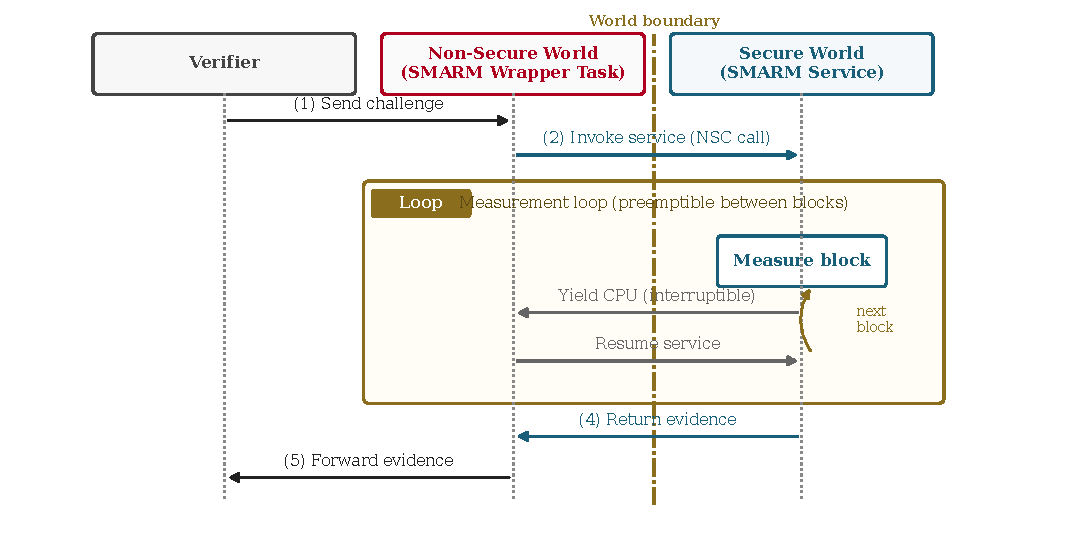
\includegraphics[width=\linewidth]{smarm_workflow.pdf}
\caption{The end-to-end workflow of our new SMARM proposal using TrustZone-M}
\label{fig:smarm_workflow}
\end{figure}

To complete this section, we describe the end-to-end interaction between the verifier and the SMARM components on the prover, as illustrated in Figure~\ref{fig:smarm_workflow}:

\begin{enumerate}
    \item The verifier sends a fresh challenge to the prover. The challenge is received by the SMARM Wrapper Task executing in the Non-Secure world; optionally, other tasks may receive the challenge and forward it to the wrapper.
    
    \item Upon receiving the challenge, the SMARM Wrapper Task invokes the SMARM Service through an NSC entry point.
    
    \item The SMARM Service executes the SMARM logic inside the Secure world, following Algorithm~\ref{alg:smarm_baseline}.
    Notably, after each block measurement completes, execution may return to the Non-Secure world, where the RTOS can preempt the SMARM Wrapper Task (which runs at the lowest priority) to schedule real-time tasks.

    \item After completing the attestation, the SMARM Service returns the attestation evidence to the SMARM Wrapper Task.
    
    \item Finally, the SMARM Wrapper Task forwards the evidence to the verifier. If the verifier receives no or invalid evidence, it treats the prover as compromised.
\end{enumerate}



\section{Evaluation of SMARM on RTOS-based Systems}
\label{sec:evaluation}

This section evaluates our TrustZone-M-based SMARM realization on RTOS platforms, focusing on implementation details, non-interruptibility behavior, and real-time availability under different workloads.

\subsection{Implementation}

We implement the new realization of SMARM on an STM32 Nucleo-144 development board~\cite{stm32l552_nucleo144}, which is equipped with an ARM Cortex-M33 MCU running at 110MHz, 512KB of flash storage, and 256KB of SRAM;
it also supports the TrustZone-M security extension.
In our configuration, 256KB of flash and \ben{96KB} of SRAM are allocated to the Secure world, with the remaining memory assigned to the Non-Secure world\ben{; the flash split is enforced by the flash secure-watermark option bytes and the SRAM split by the GTZC MPCBB (\texttt{0x20000000}--\texttt{0x20017FFF} Secure)}.


\paragraph{\ben{Attested memory region.}}
\ben{The attestation target in our threat model is the Non-Secure firmware image, which resides in the upper $256$~KiB of flash (\texttt{0x08040000}--\texttt{0x0807FFFF}).
The lower $256$~KiB holds the Secure-world image, which belongs to the TCB and is protected by TrustZone-M rather than attested.
To evaluate a larger workload, our runtime and energy benchmarks let the SMARM Service traverse the whole flash address range \texttt{0x08000000}--\texttt{0x0807FFFF} in a single shuffled traversal per attestation round, i.e., $|M| = 512$~KiB and $n = |M|/B$; all storage values are computed for the same~$n$.
SHA-256/HMAC, the PRNG, and FFX execute in time independent of the data being processed, so the cost depends only on the number of bytes hashed and on~$n$, not on which region supplies them.
Moreover, hashing dominates the per-byte cost (about $100$ cycles per byte, i.e., $481$~ms for $512$~KiB at $110$~MHz with $B = 4096$~bytes), whereas a flash word read takes only a few cycles.
Our results therefore correspond to attesting a $512$~KiB memory region.
Attesting only the $256$~KiB Non-Secure image halves~$n$ for a given~$B$: the hashing and per-block FFX costs scale linearly with~$|M|$, and the bitmap-scan cost of \rtsmarmone scales with~$n^2$.
Hence, the reported runtime, energy, and storage values are upper bounds for that deployment; for example, at $B = 1024$~bytes the SMARM permutation shrinks from $576$ to $256$~bytes.
Each attestation round in our measurements performs one shuffled traversal ($T = 1$); the cost of $T$ independent traversals scales linearly with~$T$, and Section~\ref{sec:traversals} reports the complete configuration required for a target escape probability.}


On the software side, the Non-Secure world runs an unmodified RTOS, where our prototype supports both FreeRTOS and Zephyr, compiled with size optimizations (-Os).
\ben{With FreeRTOS, the Secure world runs our bare-metal Secure image; with Zephyr, it runs TF-M, and the SMARM Service is a TF-M secure partition (Section~\ref{sec:platform-config}).}
We implement the SMARM Wrapper Task as a regular RTOS task in the Non-Secure world, consisting of \textit{115} lines of C code.
%


The Secure-world software implements the SMARM Service as detailed 
in Algorithm~\ref{alg:smarm_baseline}, where we use SHA-256 as the 
hash function for memory block measurement and HMAC-SHA256 to compute 
the attestation evidence. The Secure-world implementation consists of 
\textit{153} lines of C code and contributes \textit{33{,}968}~bytes 
to TCB.

\paragraph{\ben{Cryptographic instantiation.}}
\ben{All building blocks used by SMARM and \rtsmarm\ are instantiated as follows.
\begin{itemize}
  \item \emph{Keys and KDF.} The master key $k$ is a $256$-bit secret provisioned in Secure flash.
  $\mathsf{KDF}(\ell \,\|\, k) = \mathsf{HMAC\text{-}SHA256}(k, \ell)$ with a one-byte label $\ell \in \{\texttt{0x00}, \texttt{0x01}\}$ yields the $256$-bit keys $k_{\mathrm{prp}}$ (order generation) and $k_{\mathrm{mac}}$ (attestation MAC); no key is used for both purposes.
  \item \emph{Seed.} $\mathsf{Hash}(chal, k_{\mathrm{prp}})$ in Algorithms~\ref{alg:smarm_baseline}--\ref{alg:rtsmarm-bitarray} denotes $\mathsf{HMAC\text{-}SHA256}(k_{\mathrm{prp}}, chal)$, whose $32$-byte output is split into a $128$-bit key and a $128$-bit initial counter block.
  \item \emph{PRNG.} $\mathsf{PRNG}$ is AES-128 in counter mode under that key and counter block (the counter is incremented as a $128$-bit big-endian integer); its keystream is consumed as consecutive $32$-bit words.
  \item \emph{RandInt.} To draw a uniform integer in $[0, m)$, $\mathsf{RandInt}$ uses rejection sampling: it draws a $32$-bit word $r$, accepts it if $r < m \cdot \lfloor (2^{32}-1)/m \rfloor$, and returns $r \bmod m$. To avoid a division on the secret~$r$, the constant-time variant instead uses Lemire's multiply-high method with its corresponding rejection rule~\cite{lemire2019fast}, which is also exactly uniform (Section~\ref{sec:rtsmarm-bitarray}).
  The output is exactly uniform, and the rejection probability is below $m/2^{32} \le 2^{-19}$ for all evaluated $n \le 8192$.
  The number of rejections is independent of the returned value, so the sampling time reveals nothing about it.
  $\mathsf{PRNG.RandInt}(1, rem)$ in Algorithm~\ref{alg:rtsmarm-bitarray} is $1 + \mathsf{RandInt}(rem)$.
  \item \emph{Fisher--Yates.} SMARM generates $\sigma$ with the Durstenfeld variant of Fisher--Yates~\cite{fisherYates}: for $i = n-1$ down to $1$, it swaps positions $i$ and $\mathsf{RandInt}(i+1)$.
  \item \emph{MAC and measurement.} The evidence is $\mathsf{HMAC\text{-}SHA256}$ under $k_{\mathrm{mac}}$ over the blocks in measurement order (Assumption~\ref{asm:sha256-prf}).
\end{itemize}
The FFX instantiation of \rtsmarmtwo is specified in Section~\ref{sec:rtsmarm-fpe}.
\emph{Concrete security.} Order generation uses $128$-bit keys (AES-128 and Speck128/128), giving a $128$-bit security level against exhaustive key search, while the attestation MAC uses a $256$-bit key and a $256$-bit tag.
Beyond these generic bounds, an adversary's ability to predict the next block exceeds the inherent $1/rem$ guessing probability of a uniform shuffle only by the PRF advantage against HMAC-SHA256 and the PRP/PRF advantage against AES-128 (resp.\ FFX over Speck128/128); Appendix~\ref{sec:formal-security} makes this reduction explicit.}


\subsection{Non-interruptibility Period}

\begin{figure}[!htp]
    \centering
    \includegraphics[width=0.9\linewidth]{tdisabledplot.pdf}
   \caption{Non-interruptibility period $t_{\text{disabled}}$ of our SMARM proposal on the STM32 Nucleo-144 platform. Each point is averaged over five runs and standard deviations are below 1\%. \ben{The Secure world is our bare-metal Secure image with FreeRTOS and TF-M with Zephyr.}}
    \label{fig:tdisabled_nucleo}
\end{figure}

We first evaluate SMARM on our STM32 Nucleo-144 prototype, focusing on the non-interruptibility period $t_{\text{disabled}}$, i.e., the time spent in an atomic block measurement.
Since $t_{\text{disabled}}$ depends on the block size $B$, we consider
$B \in \{64, 128, 256, 512, 1024, 2048, 4096\}$~bytes and run SMARM using both FreeRTOS and Zephyr as the underlying RTOS.

Figure~\ref{fig:tdisabled_nucleo} reports the measured $t_{\text{disabled}}$ for each block size.
As expected, $t_{\text{disabled}}$ grows approximately linearly with $B$, confirming that larger blocks lead to longer non-interruptibility periods on our target device.
Together with the storage analysis in Figure~\ref{fig:smarm_tdisabled}, the results show that our realization preserves SMARM's original performance trade-offs~\cite{smarm}.
However, these trends do not directly reveal the impact on real-time availability, which we examine in the next subsection.



\subsection{Real-time Availability: Setup \& Metric}

\paragraph{\textbf{Experimental Setup}}
%The experiments are executed on an ARM Cortex-M33 MCU at 110MHz. 
%To ensure a fair comparison, both RTOS-based environments are compiled with size optimizations (-Os), and timing measurements are captured using the hardware cycle counter to achieve high-precision results.
To evaluate the impact of SMARM on real-time availability in RTOS-based systems, we consider a simplified yet representative scenario of real-time settings where SMARM runs alongside a single real-time task $T_{RT}$.
%\footnote{We use a single-task system a conservative baseline: if real-time availability cannot be achieved in this setting, it is unlikely to hold in more complex systems with multiple real-time tasks with different deadlines.}.

In particular, we model three classes of practical real-time workloads by varying $T_{RT}$ frequency:
\begin{enumerate}
    \item \textbf{High} real-time workload where $T_{RT}$ runs at 1000Hz
    \item \textbf{Medium} real-time workload -- 100Hz
    \item \textbf{Low} real-time workload -- 10Hz
\end{enumerate}

Although our setup includes only one real-time task, it is intentionally conservative.
Our purpose is to identify the conditions under which SMARM and real-time settings fail to co-exist.
In other words, if co-existence does not hold in this simplified setting, it is unlikely to do so in more complex deployments with multiple real-time tasks.


\ben{Table~\ref{tab:rt-task} lists the task and measurement parameters, which are identical on FreeRTOS and Zephyr.
$T_{RT}$ is a periodic task with an implicit deadline ($D = P = 1/f$).
Its jobs are released by an absolute periodic delay (\texttt{osDelayUntil} on FreeRTOS and its counterpart on Zephyr), which the kernel services on its $1$~kHz tick.
If a release time has already passed in kernel time when the previous job completes, the next job runs immediately; there is no other catch-up mechanism.
The job body is intentionally minimal: it only increments a release counter, so the utilization of $T_{RT}$ itself is negligible and FAR isolates the interference caused by attestation rather than contention between application tasks.
$T_{RT}$ runs at a higher priority than the Wrapper Task under preemptive fixed-priority scheduling, and no other application task is active.
The Wrapper Task starts the first attestation round $3$~s after boot and waits $2$~s after each round, so every round starts from an otherwise idle system; we did not vary the release phase of $T_{RT}$ relative to the start of a round.
Immediately before and after each NSC call, the Wrapper Task reads the release counter and a $32$-bit hardware timer (TIM2, clocked at $110$~MHz$/800 = 137.5$~kHz, i.e., $7.27~\mu$s resolution) that keeps counting while interrupts are masked.
$f_{\text{observed}}$ is the number of jobs of $T_{RT}$ completed in this interval divided by its duration.
We run $10$ rounds for every combination of block size, frequency, and RTOS, and each point in Fig.~\ref{fig:setup_and_baseline_far} is the mean FAR over these rounds, i.e., over about $5$--$6.5$~s of attestation.
At $10$~Hz, one round spans only about five periods of $T_{RT}$, so the per-round FAR changes in steps of about $0.2$ and the mean at this frequency is less precise than at $100$ and $1000$~Hz.}

\begin{table}[!ht]
  \centering
  \small
  \setlength{\tabcolsep}{4pt}
  \ben{%
  \begin{tabular}{@{}lp{0.58\linewidth}@{}}
    \toprule
    \textbf{Parameter} & \textbf{Value} \\
    \midrule
    Real-time task & one periodic task $T_{RT}$ \\
    Frequency $f$ (period $P$) & $1000$, $100$, $10$~Hz ($1$, $10$, $100$~ms) \\
    Deadline & implicit, $D = P$ \\
    Release & absolute periodic delay on the $1$~kHz kernel tick \\
    Job body & increment of a release counter \\
    Priorities & $T_{RT}$ above the Wrapper Task \\
    Scheduling & preemptive, fixed priority; $110$~MHz core \\
    Attestation & one round ($T = 1$), then $2$~s idle \\
    Rounds per point & $10$ \\
    Time base & TIM2 at $137.5$~kHz ($7.27~\mu$s) \\
    $f_{\text{baseline}}$ & nominal $f$ (confirmed with interrupts enabled) \\
    \bottomrule
  \end{tabular}}
  \caption{\ben{Real-time task and measurement parameters of the FAR experiments (FreeRTOS and Zephyr).}}
  \label{tab:rt-task}
\end{table}I


%, where additional scheduling contention would further reduce available slack and potentially lower FAR.
%Therefore, our results should be interpreted as an optimistic upper bound on SMARM's real-time compatibility.
%A comprehensive evaluation under multi-task workloads is left for future work.

\paragraph{\textbf{Metric}}
To quantify the impact of SMARM on real-time availability, we 
introduce the \emph{Frequency Accuracy Ratio} (FAR), defined as
\begin{equation}
    FAR = \frac{f_{\text{observed}}}{f_{\text{baseline}}}.
\end{equation}
Here, $f_{\text{observed}}$ denotes the execution frequency of 
the real-time task $T_{RT}$ when SMARM is active (including both 
the SMARM Wrapper Task and SMARM Service).
In contrast, $f_{\text{baseline}}$ denotes the baseline frequency 
of $T_{RT}$ in the absence of SMARM-induced interference, i.e., 
SMARM without disabled interrupts (Lines 5 and 7 in 
Algorithm~\ref{alg:smarm_baseline}).\ben{In this baseline configuration, $T_{RT}$ ran at its nominal frequency~$f$ (FAR $= 1.0$), so we use $f_{\text{baseline}} = f$.}
Intuitively, FAR measures how well the real-time task maintains 
its intended execution rate in the presence of SMARM.
$FAR = 1.0$ means that SMARM introduces no interference due to 
non-interruptible operations.
As these non-interruptible operations increasingly delay task 
execution, the observed frequency of $T_{RT}$ decreases, leading to a lower FAR.~\\

% However, FAR~$\approx 1.0$ alone does not guarantee full real-time compatibility.
% Instead, it should be interpreted as a \emph{necessary condition}: if FAR deviates significantly from~1.0, then no scheduling policy can ensure that $T_{RT}$ consistently meets its deadlines in the presence of SMARM.
% A complete schedulability analysis, including metrics such as deadline miss rate, response time, and worst-case execution time (WCET), is orthogonal to our current study and is left for future work.

\noindent\textbf{Remark.}
FAR does not replace schedulability analysis.
It measures the frequency-level interference caused by SMARM's non-interruptible block measurements, assuming $T_{RT}$ is already schedulable in the baseline SMARM configuration where interrupts are not disabled.
If this assumption does not hold, the problem is an orthogonal scheduling issue independent of SMARM.
\ben{FAR deliberately isolates one effect.
The remaining attestation work (order generation, $\mathsf{FindKthZero}$ or $\mathsf{FFX.Enc}$, HMAC setup and finalization, and the Wrapper Task itself) runs with interrupts enabled at the lowest application priority.
It therefore consumes only processor time left over by higher-priority tasks, apart from context-switch overhead, but it does delay any task whose priority is not above the Wrapper Task.
We quantify this total attestation work separately through the end-to-end runtime and energy in Section~\ref{sec:rtsmarm-evaluation}, and we derive the worst-case blocking that attestation adds to higher-priority tasks in Section~\ref{sec:blocking}.
FAR does not report response times, release jitter, or deadline misses.}


\begin{figure}[!ht]
    \centering
    \begin{subfigure}[t]{0.9\linewidth}
        \centering
        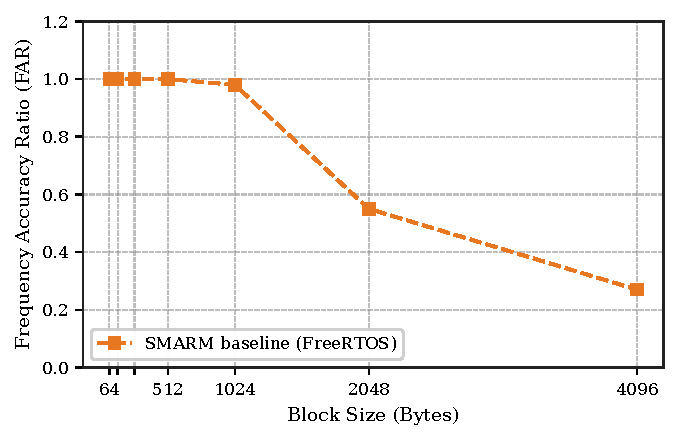
\includegraphics[width=\linewidth]{far_1000.pdf}
        \caption{High real-time workload}
        \label{fig:baseline_results_1000hz}
    \end{subfigure}
    \vspace{0.6em}
    \begin{subfigure}[t]{0.9\linewidth}
        \centering
        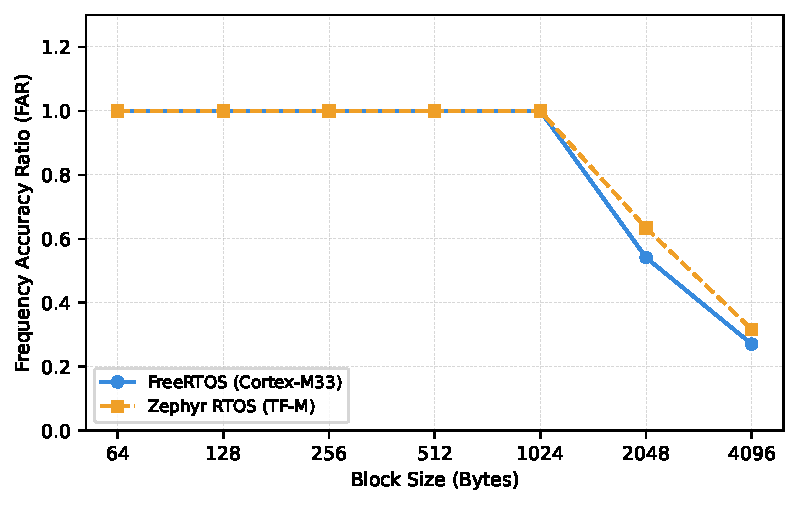
\includegraphics[width=\linewidth]{far_100.pdf}
        \caption{Medium real-time workload}
        \label{fig:baseline_results_100hz}
    \end{subfigure}
    \vspace{0.6em}
    \begin{subfigure}[t]{0.9\linewidth}
        \centering
        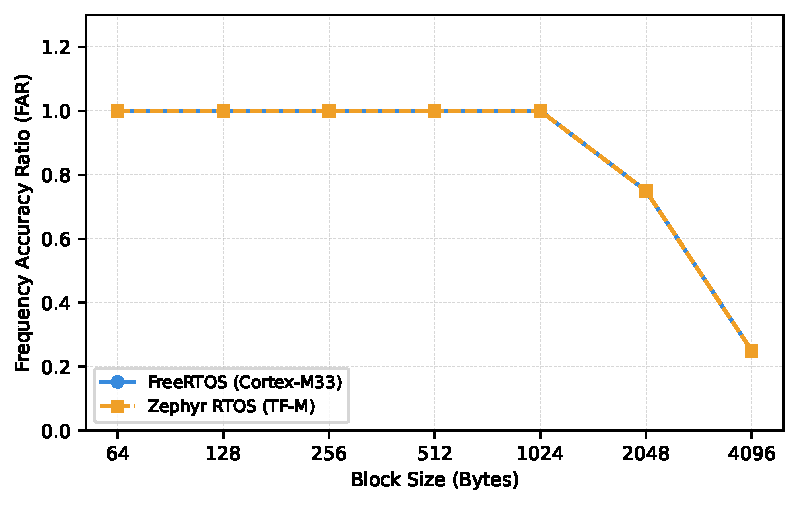
\includegraphics[width=\linewidth]{far_10.pdf}
        \caption{Low real-time workload}
        \label{fig:baseline_results_10hz}
    \end{subfigure}
    \caption{Real-time availability of SMARM under different real-time workloads}
    \label{fig:setup_and_baseline_far}
\end{figure}

\subsection{Real-time Availability: Results}

Figure~\ref{fig:setup_and_baseline_far} reports FAR across different block sizes, real-time workloads, and RTOS choices.
Across all configurations, we observe a consistent trend: FAR remains close to $1.0$ for $B \leq 1024$~bytes, but degrades noticeably as the block size increases.

At $B = 2048$~bytes, FAR decreases to approximately $0.55$ on FreeRTOS and $0.65$ on Zephyr under medium/high real-time workloads, while remaining around $0.75$ under low workloads.
At $B = 4096$~bytes, FAR drops further to $0.27$ on FreeRTOS and $0.32$ on Zephyr across all workload settings.
These results indicate that SMARM cannot reliably preserve real-time availability at these larger block sizes\ben{, at least for tasks that, like $T_{RT}$, are released by the kernel tick in our configuration}.


Both RTOS-s exhibit nearly identical FAR trends.
This suggests that the dominant source of interference is SMARM’s atomic block measurement rather than RTOS-specific scheduling behavior.
In particular, the block size $B$, which directly determines the non-interruptibility period, emerges as the primary factor affecting real-time availability.
\ben{On FreeRTOS, the position of the threshold follows from how $T_{RT}$ is released.
While a block is measured, interrupts are masked, and all SysTick interrupts that occur in this interval collapse into a single pending exception~\cite{armv8m-arm}; the kernel tick count therefore advances by at most one tick per block measurement.
If $t_{\text{disabled}}$ is shorter than the $1$~ms tick period ($0.94$~ms at $B = 1024$~bytes), no tick is lost and every job of $T_{RT}$ is released, at most $t_{\text{disabled}}$ late.
For longer blocks the kernel loses ticks, and the releases of $T_{RT}$, which follow the tick count, proceed at roughly $1~\text{ms}/t_{\text{disabled}}$ of their nominal rate, i.e., $0.53$ at $B = 2048$~bytes and $0.27$ at $B = 4096$~bytes ($t_{\text{disabled}} = 1.88$ and $3.75$~ms), which closely matches the measured FAR of $0.55$ and $0.27$.
This also explains why FAR at a given $B \ge 2048$~bytes hardly depends on the frequency of~$T_{RT}$.Zephyr, where the block is measured inside TF-M, shows the same threshold with somewhat higher FAR above it ($0.65$ and $0.32$); its $t_{\text{disabled}}(B)$ is shown separately in Fig.~\ref{fig:tdisabled_nucleo}, and we restrict the quantitative explanation above to FreeRTOS.
It is an instance of the cross-world tick loss characterized by Joia Neto et al.~\cite{joianeto2026timekeeping}, whose model predicts $\max(0, t_{\text{disabled}}/T_{\text{tick}} - 1)$ lost ticks per masked interval on average for a tick period~$T_{\text{tick}}$.
Their Secure-side tick compensation, which updates the Non-Secure kernel's tick state before interrupts are re-enabled, would release the affected jobs late instead of dropping them, but it would not shorten the blocking discussed in Section~\ref{sec:blocking}.

Two consequences limit how far the $B \le 1024$~bytes threshold generalizes.
First, it is tied to the $1$~kHz tick of our configuration: FAR~$\approx 1.0$ requires $t_{\text{disabled}}$ to stay below one tick period, so a finer tick lowers the admissible block size.
Second, FAR~$= 1.0$ does not mean that attestation causes no delay: a job may still be released up to $t_{\text{disabled}}$ late, which FAR does not capture.}

However, these results also reveal a key limitation of SMARM.
To maintain $FAR \approx 1.0$ across all evaluated settings, we must use relatively small block sizes ($B \leq 1024$~bytes).
Under SMARM, smaller blocks imply a larger number of memory partitions and therefore increased secure storage for the permutation $\sigma$, ranging from $576$~bytes at $B = 1024$~bytes to approximately $13$~KB at $B = 64$~bytes.

Such storage demands can become problematic in Secure-world deployments that must coexist with other services, such as confidential DNN inference~\cite{tslices}, control-flow integrity monitoring~\cite{tzmcfi}, or secure key storage~\cite{silabs-secure-key-storage}.
In these scenarios, dedicating between several hundred bytes and tens of kilobytes of Secure RAM solely for storing $\sigma$ may be impractical.

\subsection{\ben{Worst-Case Blocking for Schedulability Analysis}}
\label{sec:blocking}
\ben{FAR characterizes one synthetic task.
For an arbitrary task set, the effect of attestation on higher-priority tasks can instead be expressed as a blocking term in standard response-time analysis.
In SMARM and in both variants of Section~\ref{sec:resmarm-design}, interrupts are masked only while a single block is measured; order generation, including $\mathsf{FindKthZero}$ and $\mathsf{FFX.Enc}$, runs with interrupts enabled.
To the rest of the system, attestation therefore behaves as a lowest-priority task with non-preemptible sections of length at most $t_{\text{disabled}}(B)$.
A job of a higher-priority task that is released during such a section waits at most until the section ends.
It then preempts the Secure Service and is not blocked by attestation again before it completes, because the Secure Service cannot run while a higher-priority job is ready.
Under preemptive fixed-priority scheduling, the worst-case response time $R_i$ of a task $\tau_i$ with worst-case execution time $C_i$ is thus the smallest solution of
\begin{equation}
  R_i = C_i + t_{\text{disabled}}(B) + \sum_{j \in hp(i)} \left\lceil \frac{R_i}{P_j} \right\rceil C_j,
  \label{eq:rta}
\end{equation}
where $hp(i)$ is the set of tasks with a higher priority than $\tau_i$ and $P_j$ are their periods~\cite{joseph1986response,audsley1993applying,buttazzo2011hard}.
The attestation term has the same form as the blocking caused by a lower-priority non-preemptive section~\cite{sha1990priority}; in practice, it also includes a small constant exception-entry and context-switch overhead.
Hence a task set that meets its deadlines without attestation still meets them with attestation if Eq.~\eqref{eq:rta} holds for every task above the Wrapper Task.
The blocking term depends on~$B$ and the platform (Fig.~\ref{fig:tdisabled_nucleo}; e.g., $0.94$~ms at $B = 1024$~bytes on FreeRTOS), not on the scheme, because the block measurement is identical in all three schemes.
By the same argument, attestation adds at most $t_{\text{disabled}}(B)$ of release jitter to each job.
Two effects lie outside this analysis.
First, tasks released by the kernel tick additionally require $t_{\text{disabled}}(B)$ to stay below one tick period; otherwise the kernel loses ticks and its time base drifts (Section~\ref{sec:evaluation}), which Eq.~\eqref{eq:rta} does not model.
Second, the analysis covers only tasks with a priority above the Wrapper Task.
The completion time of the attestation itself grows with the load of those tasks; it can be bounded by the same recurrence, with $C$ equal to the runtime in Table~\ref{tab:runtime_overhead} and without the blocking term, and it lengthens the window of exposure discussed in Section~\ref{sec:rtsmarm-evaluation}.
These bounds are analytical; we did not measure response-time distributions, which remains future work (Section~\ref{sec:limitations}).}



\section{\rtsmarm: Reducing Secure Storage in SMARM}
\label{sec:resmarm-design}



In this section, we propose \rtsmarm, enhanced versions of SMARM that reduce secure storage requirements \ben{while satisfying the same security requirements (S1)--(S3) and retaining comparable real-time behavior, as measured by FAR}.


\rtsmarm retains the same high-level structure as SMARM, consisting of the Wrapper Task and the Secure Service.
The Wrapper Task remains unchanged, while we redesign the Secure Service to reduce the secure storage overhead.

The key idea of \rtsmarm is to trade secure storage for additional computation, thereby enabling the use of smaller block sizes under tight secure-memory budgets.
We present two variants of \rtsmarm.
The first variant, \rtsmarmone (Section~\ref{sec:rtsmarm-bitarray}), reduces the secure storage requirement from $O(n \log n)$ to $O(n)$.
The second variant, \rtsmarmtwo (Section~\ref{sec:rtsmarm-fpe}), \ben{removes the $n$-dependent permutation storage, leaving only constant-size secure state}, at the cost of significantly longer overall runtime.




\subsection{\rtsmarmone\ -- Reducing Secure Storage to $O(n)$}
\label{sec:rtsmarm-bitarray}


% \begin{algorithm}[!t]
% \caption{\rtsmarmone (secure world)}
% \label{alg:rtsmarm-bitarray}
% \begin{algorithmic}[1]
% \small
% \Notation Memory $M$, block size $B$, number of blocks $n$, key $k$, challenge $chal$
% \State \colorbox{codehl}{\textbf{for all} $i \in \{0,\dots,n-1\}$: $\text{used}[i] \gets 0$} 
%        \Comment{new: bitmap initialisation}
% \State \colorbox{codehl}{$\text{seed} \gets \mathsf{Hash}(chal, k)$}
% \State \colorbox{codehl}{$\mathsf{PRNG.Init}(\text{seed})$}
% \State \Call{HMAC.Init}{$k$}
% \For{$rm \gets 0$ to $n-1$}
%     \State \colorbox{codehl}{$\text{rem} \gets n - rm$}
%     \State \colorbox{codehl}{$r \gets \mathsf{PRNG.RandInt}(\text{1}, \text{rem})$}
%     \State \colorbox{codehl}{$idx \gets \mathsf{FindKthZero}(\text{used}, r)$}
%     \Comment{\ben{always scans all $n$ bits; no early exit}}
%     \State \colorbox{codehl}{$\text{used}[idx] \gets 1$}
%     \State \Call{DisableInterrupts}{}
%     \State \Call{HMAC.Update}{hmac, $M_{idx}$, $B$}
%     \State \Call{EnableInterrupts}{}
% \EndFor
% \State att\_evidence $\gets$ \Call{HMAC.Finalize}{hmac}
% \Output att\_evidence
% \end{algorithmic}
% \end{algorithm}
\begin{algorithm}[!t]
\caption{\rtsmarmone (secure world)}
\label{alg:rtsmarm-bitarray}
\begin{algorithmic}[1]
\small
\Notation Memory $M$, block size $B$, number of blocks $n$, master key $k$, challenge $chal$\ben{, authenticated header $\mathit{hdr}$ (Section~\ref{sec:porting})}
\State \colorbox{codehl}{\textbf{for all} $i \in \{0,\dots,n-1\}$: $\text{used}[i] \gets 0$} 
       \Comment{new: bitmap initialisation}
\State \ben{$k_{\mathrm{prp}} \gets \mathsf{KDF}(0 \,\|\, k)$}
\State \ben{$k_{\mathrm{mac}} \gets \mathsf{KDF}(1 \,\|\, k)$}
\State \colorbox{codehl}{\ben{$\text{seed} \gets \mathsf{Hash}(chal, k_{\mathrm{prp}})$}}
\State \colorbox{codehl}{$\mathsf{PRNG.Init}(\text{seed})$}
\State \ben{\Call{HMAC.Init}{$k_{\mathrm{mac}}$}; \Call{HMAC.Update}{hmac, $\mathit{hdr}$}}

\For{$rm \gets 0$ to $n-1$}
    \State \colorbox{codehl}{$\text{rem} \gets n - rm$}
    \State \colorbox{codehl}{$r \gets \mathsf{PRNG.RandInt}(\text{1}, \text{rem})$}
    \State \colorbox{codehl}{$idx \gets \mathsf{FindKthZero}(\text{used}, r)$}
           \Comment{\ben{always scans all $n$ bits; no early exit}}
    \State \colorbox{codehl}{$\text{used}[idx] \gets 1$}
    \State \Call{DisableInterrupts}{}
    \State \Call{HMAC.Update}{hmac, $M_{idx}$, $B$}
    \State \Call{EnableInterrupts}{}
\EndFor
\State att\_evidence $\gets$ \Call{HMAC.Finalize}{hmac}
\Output att\_evidence
\end{algorithmic}
\end{algorithm}

Algorithm~\ref{alg:rtsmarm-bitarray} describes the operation of the Secure Service in \rtsmarmone (note that the Wrapper Task remains unchanged).
Instead of storing the full permutation $\sigma$ to determine the measurement order, \rtsmarmone uses a bitmap \texttt{used} of size $n$ to track which memory blocks have already been measured, i.e., \texttt{used}[i] contains a bit indicating whether block $M[i]$ has been measured by \rtsmarmone.

\rtsmarmone first initializes \texttt{used} to all zeros (Line~1), indicating that no blocks have been measured.
\ben{It then derives domain-separated keys $k_{\mathrm{prp}}$ and $k_{\mathrm{mac}}$ from the master key $k$ (Lines~2--3) and initializes a PRNG using the challenge $chal$ and $k_{\mathrm{prp}}$ (Lines~4--5).}

For each measurement iteration, \rtsmarmone determines the next block to measure as follows.
It first computes the number of remaining (unmeasured) blocks, denoted as $rem$ (Line~8) and then generates a random integer $r \in [1, rem]$ (Line~9).
Since $r$ does not directly correspond to a valid block index (some blocks may have already been measured), \rtsmarmone scans the \texttt{used} bitmap to locate the $r$-th zero entry and maps it to a block index $idx$ (Line~10).

The selected block is then marked as measured by setting $\texttt{used}[idx] \leftarrow 1$ (Line~11).
Subsequently, $M_{idx}$ is measured following the same way as in SMARM.
This process repeats until all blocks have been covered, after which the attestation evidence is computed and becomes the output of the Secure Service (Line~16).


\subsubsection{Secure Storage vs.\ Runtime Trade-off.}
Compared to SMARM, \rtsmarmone replaces the secure storage of the permutation $\sigma$ with a bitmap \texttt{used}.
Since \texttt{used} contains $n$ entries, it requires $n$ bits of secure storage.
This reduces the storage requirement from $n \cdot \lceil \log_2 n \rceil$ bits in SMARM to $n$ bits in \rtsmarmone.

This reduction in storage comes at the cost of potential additional runtime overhead.
In SMARM, the permutation $\sigma$ is generated once (e.g., via \texttt{FisherYates} in Algorithm~\ref{alg:smarm_baseline}) before the measurement loop, after which each block index can be retrieved in constant time.
In contrast, \rtsmarmone determines the next block indices on-the-fly by scanning the \texttt{used} bitmap to locate the $r$-th unmeasured block.
\ben{Our implementation of $\mathsf{FindKthZero}$ always traverses all $n$ bitmap entries (a full pass, $\Theta(n)$ per iteration), rather than stopping early when the $r$-th zero is found; the wall-clock cost may depend on the public parameter $n$, but not on the secret selected index $idx$.}


\paragraph{\ben{Timing behavior of order generation.}}
\ben{Between two block measurements, KFV malware can measure how long the Secure Service runs before the next interrupt window.
In \rtsmarmone, this interval covers $\mathsf{RandInt}$, $\mathsf{FindKthZero}$, and the bitmap update.
We require its duration to depend only on public values ($n$ and the number of remaining blocks $rem$, which KFV malware knows by assumption) and on events that are independent of the selected block.
\begin{itemize}
  \item \emph{$\mathsf{FindKthZero}$.} The scan is branch-free: for each $i < n$ it computes $z = 1 - \texttt{used}[i]$, a match flag $e = [c = r-1]$ by arithmetic on $c \oplus (r-1)$, updates $idx \mathrel{|}= (-(z \cdot e)) \mathbin{\&} i$, and sets $c \gets c + z$.
  Every $i$ executes the same instruction sequence, and the bitmap resides in Secure SRAM, which is not cached on STM32L5, so the scan time is a function of~$n$ only.
  \item \emph{$\mathsf{RandInt}$.} Rejection sampling redraws a word with probability below $2^{-19}$. Because draws are independent and the accepted output is uniform, the number of rejections is independent of the output.
  To avoid an operand-dependent division on the secret word, the output is computed with the multiply-high method of Lemire~\cite{lemire2019fast}, using one constant-time $32 \times 32 \to 64$-bit multiplication. The only division is $2^{32} \bmod m$, which involves the public~$m$ only.
  \item \emph{Ciphers and hashing.} SHA-256/HMAC and Speck (an add--rotate--xor design) use no secret-indexed memory accesses.
  The table-based AES-128 used by the PRNG performs S-box lookups at secret indices; because flash reads may be served by the instruction cache, we place its tables in Secure SRAM so that every lookup has the same latency.
\end{itemize}
The evaluated prototype differs from this specification in three ways.
It uses a full-pass $\mathsf{FindKthZero}$ with data-dependent branches.
It reduces modulo~$m$ with \texttt{UDIV}.
It reads the AES tables from flash.
Its branch outcomes are determined by the number of zero entries ($rem$, public) and a single match.
On a core whose branch cost depends only on the outcome, this makes the total scan time a function of $(n, rem)$, but we do not rely on this microarchitectural property.
The constant-time forms above change only a few instructions per bitmap entry and per random word.
They leave the $\Theta(n)$ scan and the hashing cost unchanged, so the runtime results in Section~\ref{sec:rtsmarm-evaluation} remain representative.
\rtsmarmtwo is less exposed to timing leakage: FFX over Speck involves no secret-dependent branches or memory accesses, and cycle walking, whose iteration count is the only data-dependent quantity, never occurs for $n$ a power of two.}

Consequently, while \rtsmarmone reduce secure storage to $O(n)$, it introduces additional per-block computation, which can increase the overall attestation runtime, especially for large $n$.



\subsubsection{Soundness.}\label{subsubsec:v1-sound}
We first establish the soundness of \rtsmarmone, i.e., showing that \rtsmarmone is functionally equivalent to SMARM.
In this context, soundness requires that (1) all memory blocks are measured exactly once, and (2) the order of block selection is randomized.

For (1), in each iteration, the algorithm selects an index $idx$ such that \texttt{used}[idx] = 0, and then sets it to $1$.
Since each iteration flips exactly one bit from $0$ to $1$, and there are $n$ such bits, after $n$ iterations all entries in \texttt{used} are set to $1$.
This means that every block is selected exactly once, and no block is measured more than once.

For (2), randomness follows from the use of PRNG seeded with the secret (random) key $k$.
At each iteration, \rtsmarmone samples a uniform random integer $r \in [1, rem]$.
The mapping from $r$ to the $r$-th zero entry in \texttt{used} establishes a one-to-one correspondence between $r$ and the set of remaining blocks.
Therefore, each unmeasured block is selected with equal probability at each step.
As a result, the overall measurement order is a uniformly random permutation over all $n$ blocks.

\subsubsection{Security}
Here, we provide informal arguments that \rtsmarmone \ben{satisfies the same security requirements (S1)-(S3) as SMARM,} defined in Section~\ref{sec:background}; we refer to Appendix~\ref{sec:proof-prng} for a formal (reduction-based) security proof of \rtsmarmone.

\begin{itemize}
  \item[(S1)] \emph{Controlled execution.}
  Recall in Section~\ref{sec:porting} that SMARM guarantees (S1) by (i) relying on TrustZone-M to restrict entry into the Secure world to well-defined entry points (Section~\ref{subsec:tzm}), and (ii) disabling interrupts during each block measurement to ensure atomic execution.
  \rtsmarmone preserves both design choices by implementing its logic as a Secure-world service and maintaining interrupt disablement during block measurement.
  Therefore, (S1) is directly inherited in \rtsmarmone.

  \item[(S2)] \emph{Key secrecy.}
  \rtsmarmone does not expose the master key $k$ or the derived keys $k_{\mathrm{prp}}$ and $k_{\mathrm{mac}}$.
  As in SMARM, these keys are stored and accessed exclusively within the Secure world.
  Hence, \rtsmarmone preserves (S2).

  \item[(S3)] \emph{Private measurement order.}
  In \rtsmarmone, the measurement order is implicitly determined by the \texttt{used} bitmap, which resides in Secure RAM inaccessible to the Non-Secure world where KFV malware may reside.
  \ben{The between-block continuation invariant of Section~\ref{sec:porting} applies with order-related Secure state consisting of the \texttt{used} bitmap, the PRNG state, the HMAC context, and the iteration index.}
  \ben{While direct access is prevented, KFV malware may attempt to infer the order via timing side channels.
  To mitigate this, we ensure that block-index selection is independent of secret-dependent early exits.
  In particular, we implement $\mathsf{FindKthZero}$ (Line~10 of Algorithm~\ref{alg:rtsmarm-bitarray}) such that it always scans all $n$ entries of the \texttt{used} bitmap, rather than terminating early upon finding the $r$-th zero.
  As a result, its execution time is independent of the selected index $idx$, ensuring that the procedure does not leak information about the measurement order through timing.}
  Replay attacks are also mitigated in the same way as in SMARM since the block order depends on a one-time challenge $chal$ and a secret $k$.
\end{itemize}



% \subsection{\rtsmarmtwo\ -- Eliminating Secure Storage}
\subsection{\rtsmarmtwo\ -- \ben{Constant-Size Secure Storage}}
\label{sec:rtsmarm-fpe}


We observe that SMARM instantiates PRP using the Fisher--Yates shuffle~\cite{fisherYates}, which produces a random permutation over $n$ elements.
While Fisher--Yates is time-efficient (i.e., in $O(n)$), it requires materializing the entire permutation, resulting in $O(n \log n)$ bits of secure storage in SMARM.


In \rtsmarmtwo, we \ben{remove this $n$-dependent storage} by instead instantiating the PRP using format-preserving encryption (FPE)~\cite{bellare2009format,ff1}.

FPE is a symmetric encryption primitive that preserves the domain of its inputs, i.e., for a given encryption key from the set $\mathcal{K}$ and a given finite domain $\mathcal{D}$, it defines an encryption as:
\[
\mathsf{FPE.Enc}: \mathcal{K} \times \mathcal{D} \rightarrow \mathcal{D}
\]
By construction, $\mathsf{FPE.Enc}$ realizes a bijection over $\mathcal{D}$, and thus directly serves as a PRP.

\begin{algorithm}[!t]
\caption{\rtsmarmtwo (secure world)}
\label{alg:rtsmarm-fpe}
\begin{algorithmic}[1]
\small
\Notation Memory $M$, block size $B$, number of blocks $n$, master key $k$, challenge $chal$\ben{, authenticated header $\mathit{hdr}$ (Section~\ref{sec:porting})}

\State \ben{$k_{\mathrm{prp}} \gets \mathsf{KDF}(0 \,\|\, k)$}
\State \ben{$k_{\mathrm{mac}} \gets \mathsf{KDF}(1 \,\|\, k)$}
\State \colorbox{codehl}{\ben{$(\text{ffx\_key}, \text{tweak}) \gets \mathsf{KDF}(k_{\mathrm{prp}}, chal)$}}
\State \colorbox{codehl}{$\mathsf{FFX.Init}(\text{ffx\_key, tweak})$}
\State \ben{\Call{HMAC.Init}{$k_{\mathrm{mac}}$}; \Call{HMAC.Update}{hmac, $\mathit{hdr}$}}
\For{$i \gets 0$ to $n-1$}
    \State \colorbox{codehl}{$idx \gets \mathsf{FFX.Enc}(i)$}
    \State \Call{DisableInterrupts}{}
    \State \Call{HMAC.Update}{hmac, $M_{idx}$, $B$}
    \State \Call{EnableInterrupts}{}
\EndFor
\State att\_evidence $\gets$ \Call{HMAC.Finalize}{hmac}
\Output att\_evidence
\end{algorithmic}
\end{algorithm}

In \rtsmarmtwo, we instantiate FPE using the FFX construction~\cite{bellare2010ffx}.
FFX implements FPE using a Feistel network~\cite{hoang2010generalized}, where each round function can be realized as a block cipher.
To keep the design lightweight, we use Speck~\cite{speck}, a block cipher optimized for efficient software execution on resource-limited platforms, which aligns with our target deployment setting.


\paragraph{\ben{FFX instantiation.}}
\ben{We instantiate FFX with the radix-2 round structure of FF1~\cite{ff1}, itself an FFX instantiation, using Speck in place of AES:
\begin{itemize}
  \item \emph{Key and tweak.} In Line~3 of Algorithm~\ref{alg:rtsmarm-fpe}, $\text{ffx\_key}$ is the first $16$ bytes of $\mathsf{HMAC\text{-}SHA256}(k_{\mathrm{prp}}, chal)$, so every attestation uses a fresh FFX key; the $32$-bit tweak is the first four bytes of $chal$ (tweaks are public in FPE).
  \item \emph{Domain encoding.} Let $\ell = \lceil \log_2 n \rceil$. The index $i \in [0, n)$ is encoded as an $\ell$-bit string and split into $A$ (the high $u = \lfloor \ell/2 \rfloor$ bits) and $B$ (the low $v = \ell - u$ bits).
  \item \emph{Rounds.} FFX applies $10$ Feistel rounds. In round $j \in \{0,\dots,9\}$, with $m = u$ for even $j$ and $m = v$ for odd $j$, it computes $y$ as the first $32$ bits of $\mathrm{CBC\text{-}MAC}_{\text{ffx\_key}}(P \,\|\, Q_j)$, where $P$ encodes the fixed parameters (radix, $\ell$, tweak length) and $Q_j$ encodes the tweak, $j$, and $B$; it then sets $(A, B) \gets (B, (A + y) \bmod 2^m)$.
  \item \emph{Block cipher.} The CBC-MAC uses Speck128/128: $128$-bit block, $128$-bit key, $64$-bit words, rotation amounts $(8, 3)$, and the full $32$ rounds~\cite{speck}. Each FFX evaluation therefore costs $10$ CBC-MAC computations.
  \item \emph{Cycle walking.} If the output is $\ge n$, FFX is re-applied under the same key and tweak until the result lies in $[0, n)$, which preserves bijectivity. In our evaluation $n = |M|/B$ is always a power of two, so cycle walking never occurs.
\end{itemize}
We do not claim conformance with SP~800-38G: Speck is not an approved block cipher, and our domains ($2^{7}$--$2^{13}$) satisfy the mandatory minimum of $100$ but are smaller than the one million that SP~800-38G recommends~\cite{ff1}.
That recommendation targets plaintext-guessing and small-domain message-recovery attacks, which require access to FPE ciphertexts~\cite{hoang2018curse}.
In \rtsmarmtwo, the FFX outputs (block indices) are never revealed outside the Secure world, and each FFX key is used for a single traversal. An adversary therefore obtains no ciphertexts, and its chance of predicting the next block remains $1/rem$ up to the PRP advantage against FFX.}


Algorithm~\ref{alg:rtsmarm-fpe} describes how \rtsmarmtwo integrates FFX into the block measurement process.
\ben{First, \rtsmarmtwo derives domain-separated keys $k_{\mathrm{prp}}$ and $k_{\mathrm{mac}}$ from the master key $k$ (Lines~1--2), then derives the FFX key and tweak from $k_{\mathrm{prp}}$ and the challenge $chal$ (Line~3), and initializes the FFX instance accordingly (Line~4). HMAC uses $k_{\mathrm{mac}}$ (Line~5).}


During the $i$-th iteration, \rtsmarmtwo determines the next block to measure by using the instantiated FFX to encrypt $i$ (Line~7).
The resulting $idx$ is then used to retrieve and measure the corresponding memory block, following the same procedure as in SMARM.
After all blocks have been measured, \rtsmarmtwo computes and returns the attestation evidence in the same manner as SMARM.

\subsubsection{Secure Storage vs.\ Runtime Trade-off.}
\ben{\rtsmarmtwo does not store any per-block permutation state in secure memory.
Its remaining secure state is constant-size and independent of~$n$: the FFX key material (including the precomputed Speck round keys) and tweak, the HMAC context, and the loop index.
Hence, \rtsmarmtwo does not eliminate secure storage; it makes the secure storage independent of~$n$.}


\ben{This removal of permutation storage} comes at the cost 
of additional per-block (non-atomic) computation.
In SMARM, each block index is retrieved in constant time 
from the pre-computed $\sigma$.
In \rtsmarmone, each iteration requires an $O(n)$ scan of 
the \texttt{used} bitmap.
In \rtsmarmtwo, each iteration invokes 
$\mathsf{FFX.Enc}$, which performs one FPE encryption using Speck as the underlying round function. 
While this operation does not depend on $n$, i.e., $O(1)$ runtime complexity, this operation is more complex than the scan operation in \rtsmarmone, potentially making its runtime longer for a smaller $n$.

Consequently, \rtsmarmtwo trades all permutation storage 
for a constant per-block cryptographic cost, making it 
the most storage-efficient variant at the expense of higher per-block computation compared to SMARM.

\subsubsection{Soundness.}
Similar to Section~\ref{subsubsec:v1-sound}, we argue the soundness by showing that in \rtsmarmtwo, (1) all memory blocks are measured exactly once, and (2) the order of block selection is randomized.

\rtsmarmtwo iterates over $i \in \{0, \ldots, n-1\}$ 
and maps each $i$ to a block indices 
$idx = \mathsf{FFX.Enc}(i)$.
Since $\mathsf{FFX.Enc}$ implements a bijection over the domain 
$\{0, \ldots, n-1\}$, each value of $idx$ is distinct for 
distinct values of $i$.
Therefore, every block is measured exactly once and no block 
is measured more than once, fulfilling (1).

(2) directly follows from the fact that FFX instantiates pseudo-random permutation and the order of block selection in \rtsmarmtwo is simply\[
  \{\mathsf{FFX.Enc}(0), \mathsf{FFX.Enc}(1), \ldots,
    \mathsf{FFX.Enc}(n-1)\},
\] making it a uniformly random permutation over all $n$ blocks.



\subsubsection{Security}
We informally argue how \rtsmarmtwo satisfies (S1)-(S3) (in Section~\ref{sec:background}) while providing a formal reduction proof in Appendix~\ref{sec:proof-fpe}.

\begin{itemize}
  \item[(S1)] \emph{Controlled execution.}
  \rtsmarmtwo preserves both design choices of SMARM for 
  enforcing (S1): it implements its logic as a Secure-world 
  service accessible only via TrustZone-M NSC entry points 
  (Section~\ref{subsec:tzm}), and it disables interrupts 
  during each block measurement via the \texttt{CPSID} 
  instruction to ensure atomic execution.
  Therefore, (S1) is directly inherited in \rtsmarmtwo.

  \item[(S2)] \emph{Key secrecy.}
   \rtsmarmtwo stores the master key $k$ and all derived material ($k_{\mathrm{prp}}$, $k_{\mathrm{mac}}$, and the FFX key/tweak) exclusively in the Secure world.
  Hence, \rtsmarmtwo preserves (S2).


  \item[(S3)] \emph{Private measurement order.}
  In \rtsmarmtwo, the measurement order is determined by 
  $\mathsf{FFX.Enc}$, whose output depends on the 
  secret key $k$ and the one-time challenge $chal$.
  Since $k$ resides exclusively in Secure RAM inaccessible to the Non-Secure world, KFV malware cannot compute or predict the permutation. \ben{ The between-block continuation invariant of Section~\ref{sec:porting} applies with order-related Secure state consisting of the FFX key and tweak, the iteration index, and the HMAC context.}

  %
  %Although FFX may be vulnerable to small-domain attacks when an adversary can observe or query multiple plaintext-ciphertext pairs~\cite{hoang2018curse}, such conditions do not arise in our setting.
  %Specifically, \rtsmarmtwo does not expose the ciphertext outputs (i.e., $idx$), nor does it provide oracle access to the underlying FFX construction.

\end{itemize}





\section{Evaluation of \rtsmarm on RTOS Systems}
\label{sec:rtsmarm-evaluation}

In this section, we evaluate the two \rtsmarm variants against the
baseline SMARM along three dimensions: secure storage 
size \ben{(permutation state and the complete measured Secure memory footprint)}, overall attestation runtime, and energy consumption. We reuse the experimental setup and FAR metric
introduced in Section~\ref{sec:evaluation}. 
As established in Section~\ref{sec:evaluation} that FreeRTOS and Zephyr exhibit similar results in SMARM, our experiments here therefore focus only on FreeRTOS.

\subsection{Secure Storage}
\label{sec:storage-runtime-tradeoff}

\begin{figure}[!ht]
    \centering
    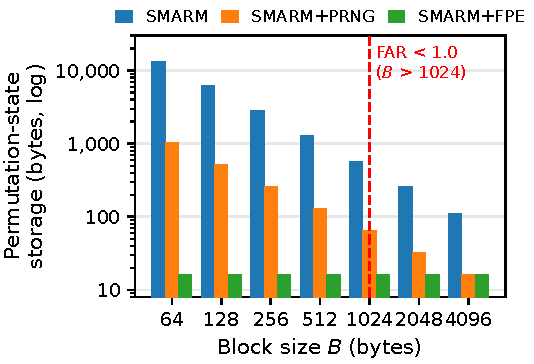
\includegraphics[width=0.95\linewidth]{fig_storage.pdf}
    \caption{\ben{Analytical permutation-state storage for $|M| = 512$~KiB with varying block sizes: bit-packed $\sigma$ ($n\lceil\log_2 n\rceil$ bits) for SMARM, the bitmap \texttt{used} ($n$ bits) for \rtsmarmone, and the $16$-byte FFX key for \rtsmarmtwo. Constant-size state (e.g., HMAC context, PRNG state, Speck round keys, stack) is excluded.} The dashed red line marks $B = 1024$~bytes, beyond which 
    FAR drops below~1.0.}
    \label{fig:storage_tradeoff}
\end{figure}


\begin{table}[!ht]
  \centering
  \small
  \setlength{\tabcolsep}{6pt}
  \begin{tabular}{rrrr}
    \toprule
    & \multicolumn{3}{c}{\textbf{Runtime (ms)}} \\
    \cmidrule(lr){2-4}
    $B$ \textbf{(bytes)} 
    & \textbf{SMARM} 
    & \textbf{\rtsmarmone} 
    & \textbf{\rtsmarmtwo} \\
    \midrule
    64    & 644 & 9{,}310 & 4{,}229 \\
    128   & 562 & 2{,}730 & 2{,}325 \\
    256   & 521 & 1{,}066 & 1{,}423 \\
    512   & 500 &   630   &   945   \\
    \rowcolor{gray!15}
    1024  & 490 &   526   &   726   \\
    2048  & 484 &   494   &   611   \\
    4096  & 481 &   484   &   553   \\
    \bottomrule
  \end{tabular}
  % \caption{Overall attestation runtime of SMARM baseline and the two \rtsmarm\ variants. The shaded row ($B = 1024$~bytes) marks $B=1024$~bytes, beyond which FAR drops below 1.0.}
    \caption{\ben{Overall attestation runtime of one shuffled traversal over $|M| = 512$~KiB (\texttt{0x08000000}--\texttt{0x0807FFFF}) under SMARM and \rtsmarm\ (FreeRTOS, no real-time task, mean over $10$ rounds). The shaded row marks $B = 1024$~bytes, beyond which FAR drops below 1.0.}}

  \label{tab:runtime_overhead}
\end{table}

Figure~\ref{fig:storage_tradeoff} compares the \ben{permutation-state} storage requirements of SMARM and both \rtsmarm variants across different block sizes $B$.
\ben{Storage is determined by the number of blocks $n = |M|/B$ with $|M| = 512$~KiB.
These values are computed analytically and count only the secret state that encodes the measurement order, i.e., the state that grows with~$n$ in SMARM and \rtsmarmone, and the FFX key from which \rtsmarmtwo derives the order.
Constant-size state that does not depend on~$n$, such as the HMAC context, the PRNG state, the expanded Speck key schedule, and the stack, is not included in Fig.~\ref{fig:storage_tradeoff}.
Our \rtsmarmone prototype stores \texttt{used} as a bit-packed array, matching the analysis.
Our SMARM prototype stores $\sigma$ as an array of 32-bit integers ($4n$ bytes); the bit-packed value in Fig.~\ref{fig:storage_tradeoff} is therefore a lower bound for SMARM and favors the baseline.}
Both \rtsmarm schemes substantially reduce secure storage overhead relative to SMARM across all evaluated configurations.

The magnitude of reduction varies across the two variants as $B$ changes.
For \rtsmarmone, the storage benefit is greater when $n$ is large (equivalently, when $B$ is small).
% For example, \rtsmarmone achieves a $13\times$ reduction at $B = 64$~bytes ($13{,}312 \rightarrow 1{,}024$~bytes), while the reduction decreases to approximately $7\times$ at $B = 4096$~bytes ($112 \rightarrow 16$~bytes).
For example, \rtsmarmone achieves a $13\times$ reduction at $B = 64$~bytes ($13{,}312 \rightarrow 1{,}024$~bytes), while the reduction decreases to approximately $7\times$ at $B = 4096$~bytes ($112 \rightarrow 16$~bytes). This trend arises because both \rtsmarmone and SMARM's storage requirements scale with $n$, albeit with different asymptotic costs.

In contrast, \rtsmarmtwo requires a fixed \ben{permutation-state} footprint of only $16$~bytes \ben{(the FFX key)}, independent of $B$/$n$.
As a result, it achieves increasingly larger reductions as $B$ decreases.
At $B = 64$~bytes, \rtsmarmtwo provides an $832\times$ reduction compared to SMARM, far exceeding the reduction achieved by \rtsmarmone.
As $B$ increases, however, the relative benefit becomes narrower, and both variants provide comparable storage savings at large block sizes such as $B = 4096$~bytes.

% At the largest block size that still achieves 1.0 FAR ($B = 1024$~bytes), \rtsmarmone reduces the storage requirement from $576$~bytes to $64$~bytes, corresponding to a $9\times$ reduction.
% \rtsmarmtwo further lowers the requirement to $16$~bytes, achieving approximately a $36\times$ reduction relative to SMARM.
At the largest block size that still achieves 1.0 FAR ($B = 1024$~bytes), \rtsmarmone reduces the \ben{permutation-state} storage requirement from $576$~bytes to $64$~bytes, corresponding to a $9\times$ reduction.
\rtsmarmtwo further lowers the requirement to $16$~bytes, achieving approximately a $36\times$ reduction relative to SMARM.
\ben{These ratios refer to permutation state only; the constant-size state excluded above adds the same HMAC and stack cost to every scheme, plus scheme-specific cipher state.
Section~\ref{sec:footprint} reports the complete measured footprint.}

\subsection{\ben{Measured Secure Memory Footprint}}
\label{sec:footprint}

\begin{table}[!ht]
  \centering
  \small
  \setlength{\tabcolsep}{4pt}
  \ben{%
  \begin{tabular}{lrrr}
    \toprule
    \textbf{Component (bytes)} & \textbf{SMARM} & \textbf{\rtsmarmone} & \textbf{\rtsmarmtwo} \\
    \midrule
    \multicolumn{4}{l}{\emph{Secure flash (attestation path)}} \\
    Code (NSC entry, order gen., HMAC, cipher) & 2{,}100 & 2{,}128 & 2{,}704 \\
    Constant tables and key & 538 & 538 & 55 \\
    \midrule
    \multicolumn{4}{l}{\emph{Secure RAM}} \\
    HMAC context (static) & 232 & 232 & 232 \\
    Cipher state (static) & -- & -- & 628 \\
    Permutation state (static) & $4n$ & $n/8$ & -- \\
    Worst-case stack & 1{,}024 & 1{,}016 & 760 \\
    Preemption frame (NS interrupt) & 72 & 72 & 72 \\
    \midrule
    Peak RAM, $B = 64$ ($n = 8192$) & 34{,}096 & 2{,}344 & 1{,}692 \\
    \rowcolor{gray!15}
    Peak RAM, $B = 1024$ ($n = 512$) & 3{,}376 & 1{,}384 & 1{,}692 \\
    Peak RAM, $B = 4096$ ($n = 128$) & 1{,}840 & 1{,}336 & 1{,}692 \\
    \bottomrule
  \end{tabular}}
  \caption{\ben{Measured Secure-world footprint of the attestation path, from the evaluated Secure builds (GCC~13.3.1, \texttt{-Os}). Code and static data are taken from the ELF symbol table; worst-case stack is the maximum over the call graph of the per-function frames reported by \texttt{-fstack-usage}. Code, stack, and cipher state do not depend on~$B$; only the permutation state does.}}
  \label{tab:footprint}
\end{table}

\ben{Fig.~\ref{fig:storage_tradeoff} isolates the permutation state.
To account for all Secure memory used by attestation, Table~\ref{tab:footprint} reports the footprint measured on the evaluated Secure builds.
We obtained code and static data from the ELF symbol table.
We obtained the worst-case stack by combining the per-function frame sizes emitted by GCC (\texttt{-fstack-usage}) with the call graph extracted from the disassembly; the call graph contains no recursion, and its only indirect call (Speck's dispatch to a variant-specific encryption routine) is bounded by the largest possible target.
\begin{itemize}
  \item \emph{Common state.} All schemes keep a $232$-byte HMAC-SHA256 context in static Secure RAM.
  The deepest stack path of every scheme is the HMAC key setup (\texttt{hmac\_sha256\_initialize} $\rightarrow$ \texttt{sha256\_update}), whose SHA-256 message schedule alone takes a $592$-byte frame.
  When a Non-Secure interrupt preempts the Secure Service between blocks, the core additionally stacks a $72$-byte exception frame with the additional state context onto the Secure stack~\cite{armv8m-arm}.
  \item \emph{SMARM and \rtsmarmone.} The AES-128 context ($176$-byte round keys plus counter block) is allocated on the Secure stack and is therefore included in the worst-case stack.
  The AES S-boxes and round constants account for $523$ of the $538$ bytes of constant tables.
  SMARM stores $\sigma$ as \texttt{int indices[n]} ($4n$ bytes); \rtsmarmone stores the bit-packed bitmap ($n/8$ bytes).
  \item \emph{\rtsmarmtwo.} The only $n$-independent secret is the $16$-byte FFX key, but its expanded form is not.
  Our Speck implementation reserves a generic $576$-byte key-schedule buffer (sized for the largest Speck variant) within a $628$-byte cipher object, of which Speck128/128 uses $256$ bytes.
  A Speck128/128-only schedule would reduce this state to about $300$ bytes.
\end{itemize}
The complete Secure images occupy about $33$--$34$~KB of flash, of which the attestation path takes $2.6$--$2.8$~KB; the remainder is the vendor HAL, startup code, FreeRTOS Secure-context support, and debug UART output, and is common to all schemes.
The attestation runs on the calling task's Secure-context stack, allocated from the Secure heap ($4{,}096$ bytes in our configuration), which exceeds the worst-case stack of every scheme.}

\ben{Two observations follow.
First, with all state included, SMARM's footprint is dominated by $\sigma$ whenever $n$ is large ($34$~KB at $B = 64$), whereas both \rtsmarm variants stay below $2.4$~KB at every evaluated block size.
Second, the ranking between the variants depends on~$B$.
Because \rtsmarmtwo carries the constant Speck state, it has the smaller peak RAM only for $B \le 128$~bytes ($n \ge 4096$).
At the operating point $B = 1024$~bytes, \rtsmarmone needs $1{,}384$~bytes, \rtsmarmtwo needs $1{,}692$~bytes, and SMARM needs $3{,}376$~bytes, i.e., $2.4\times$ and $2.0\times$ reductions in total Secure RAM.
The permutation-state ratios of Fig.~\ref{fig:storage_tradeoff} ($9\times$ and $36\times$) therefore describe how the schemes scale with~$n$, not their total footprint at moderate~$n$.}




\begin{figure}[!ht]
    \centering
    \includegraphics[width=0.95\linewidth]{fig_runtime_overhead.pdf}
    \caption{Overall runtime overhead of \rtsmarmone and \rtsmarmtwo relative to SMARM baseline across block sizes. The dashed red line marks $B = 1024$~bytes, beyond which 
    FAR drops below~1.0.}
    \label{fig:runtime_overhead}
\end{figure}

\subsection{Overall Attestation Runtime}
% Figure~\ref{fig:runtime_overhead} presents the runtime overhead of \rtsmarmone and \rtsmarmtwo relative to SMARM (when executed without interruption), while the corresponding absolute runtimes are reported in Table~\ref{tab:runtime_overhead}.
% The results show that both variants introduce additional runtime compared to SMARM, with the overhead becoming more pronounced as the block size $B$ decreases.
Figure~\ref{fig:runtime_overhead} presents the runtime overhead of \rtsmarmone and \rtsmarmtwo relative to SMARM (when executed without interruption), while the corresponding absolute runtimes are reported in Table~\ref{tab:runtime_overhead}.
\ben{As stated in Section~\ref{sec:evaluation}, these end-to-end times correspond to one shuffled traversal over $|M| = 512$~KiB.
Changing $B$ changes $n = |M|/B$ and the per-block work, but not the number of bytes attested in one round.}
\paragraph{\ben{Window of exposure.}}
\ben{End-to-end attestation latency also has a security interpretation: until a round completes and the verifier accepts fresh evidence, software compromise on the prover may remain undetected.
For example, at $B = 1024$~bytes a full round takes $490$~ms under SMARM and $726$~ms under \rtsmarmtwo, whereas \rtsmarmone at $B = 64$~bytes takes $9.3$~s.
Parameter choices that inflate total attestation time (e.g., very small $B$ under \rtsmarmone) therefore widen this window of exposure, even when FAR remains close to~$1.0$.}
The results show that both variants introduce additional runtime compared to SMARM, with the overhead becoming more pronounced as the block size $B$ decreases.



In most cases, \rtsmarmtwo tends to incur higher runtime overhead than \rtsmarmone due to the need to perform an FPE operation for each block selection.
However, for very small block sizes ($B = 64$ or $128$~bytes), \rtsmarmone becomes slower.
This is because its bitmap-based block selection requires scanning $O(n)$ entries per iteration, where $n$ grows inversely with $B$.
As a result, the cumulative scan cost becomes dominant for small blocks, leading to large overhead (e.g., $13.5\times$ of SMARM runtime at $B = 64$~bytes).
This makes \rtsmarmone less suitable for settings requiring very small block sizes.

At $B = 1024$~bytes, \rtsmarmone incurs only a moderate runtime increase of $7\%$ (526~ms vs.\ 490~ms).
For this configuration, the bitmap scan contributes little to the total execution time, which is largely dominated by hashing and HMAC-SHA256 computation over memory blocks.
%
In comparison, \rtsmarmtwo incurs around $48\%$ overhead (726~ms vs.\ 490~ms).

\subsection{Energy Consumption}
\label{sec:energy}


\begin{table}[!ht]
  \centering
  \small
  \setlength{\tabcolsep}{5pt}
  \resizebox{\linewidth}{!}{%
  \begin{tabular}{rrrr}
    \toprule
    & \multicolumn{3}{c}{\textbf{Board-level Energy (mJ)}} \\
    \cmidrule(lr){2-4}
    $B$ \textbf{(bytes)}
    & \textbf{SMARM}
    & \textbf{\rtsmarmone}
    & \textbf{\rtsmarmtwo} \\
    \midrule
    64    & 190.2 & 2{,}650 & 1{,}243 \\
    128   & 168.0 &    780  &    700  \\
    256   & 155.2 &    310  &    425  \\
    512   & 148.6 &    183  &    289  \\
    \rowcolor{gray!15}
    1024  & 145.2 &    153  &    221  \\
    2048  & 143.3 &    144  &    187  \\
    4096  & 141.0 &    141  &    170  \\
    \bottomrule
  \end{tabular}%
  }
  \caption{Board-level energy consumption per attestation round \ben{(one shuffled traversal, $T = 1$, over $|M| = 512$~KiB; gross board energy, mean over $10$ rounds)}; the shaded row marks $B = 1024$\,bytes, the largest block size preserving FAR\,$\approx$\,1.0.}
  \label{tab:energy}
\end{table}

We measure board-level energy per attestation round using 
an FNIRSI FNB58 USB power meter in series between the host 
PC and the NUCLEO-L552ZE-Q board, sampling at 100~Hz. \ben{The meter sits on the $5$~V USB supply of the board, so the measurement covers the whole board, including the on-board ST-LINK debugger.
According to its manufacturer, the meter uses a $16$-bit ADC with an accuracy of $\pm(0.02\%$ of reading $+\,2$ digits$)$ for voltage and $\pm(0.05\%$ of reading $+\,2$ digits$)$ for current~\cite{fnb58}; we rely on this specification and did not calibrate the meter against a reference instrument.
We integrate the recorded power $V \cdot I$ between the \textsc{Attest\_Start} and \textsc{Attest\_End} markers that the Wrapper Task prints over UART immediately before and after the NSC call.
Aligning these markers with the meter trace is accurate to one sample ($10$~ms) at each end.
At the observed board power of about $0.29$~W ($5.02$~V, $57$--$58$~mA), this corresponds to at most about $\pm 6$~mJ per round, or $4\%$ of the smallest value in Table~\ref{tab:energy}, which dominates the meter's own error.
We report gross board energy and do not subtract the idle draw.
Because the board draws nearly constant power in all configurations, the reported energy is approximately proportional to the attestation runtime, and differences between schemes reflect runtime differences rather than differences in instantaneous power.
Each value is the mean over $10$ consecutive rounds on FreeRTOS, with $T_{RT}$ active at $1000$~Hz.
The runtimes in Table~\ref{tab:runtime_overhead} are also means over $10$ rounds, but they were measured without $T_{RT}$ using the TIM2 time base described in Section~\ref{sec:evaluation}; for SMARM, the minimum and maximum runtime over the $10$ rounds differ by at most $3$~ms ($0.5\%$, at $B = 64$~bytes).}

% OAK: too much info below
%Energy is integrated between \textsc{Attest\_Start} and 
%\textsc{Attest\_End} UART markers, with timestamp alignment 
%within~10\,ms. The measured supply is 5.02\,V at 57--58\,mA, 
%yielding a constant board-level power draw of 288--293\,mW 
%across all configurations; energy therefore scales directly 
%with runtime.
%
Results are reported in Table~\ref{tab:energy}.
SMARM shows only small energy variation across block sizes $B$, from 190~mJ at $B=64$ to 141~mJ at $B=4096$.
In contrast, both \rtsmarm variants show stronger dependence on~$B$: 
at $B = 64$, \rtsmarmone consumes 2{,}650~mJ 
(13.9$\times$ SMARM) due to its $O(n)$ bitmap scan, 
while \rtsmarmtwo consumes 1{,}243~mJ (6.5$\times$) 
from per-block \textsf{FFX.Enc} calls.
At the operating point $B = 1024$~bytes, overhead 
narrows to $5\%$ for \rtsmarmone (153~mJ) and 
$52\%$ for \rtsmarmtwo (221~mJ).
%The variants also exhibit a crossover: \rtsmarmtwo is 
%more energy-efficient at $B \leq 128$~bytes 
%(700~mJ vs.\ 780~mJ at $B = 128$), whereas 
%\rtsmarmone is preferable at $B \geq 256$~bytes.


\subsection{\ben{Number of Traversals and Complete Configuration}}
\label{sec:traversals}

\begin{table}[!ht]
  \centering
  \small
  \setlength{\tabcolsep}{3.5pt}
  \ben{\resizebox{\linewidth}{!}{%
  \begin{tabular}{rrrrrrrr}
    \toprule
    & & \multicolumn{3}{c}{\textbf{Runtime (s)}} & \multicolumn{3}{c}{\textbf{Energy (J)}} \\
    \cmidrule(lr){3-5}\cmidrule(lr){6-8}
    $T$ & \textbf{Escape} & \textbf{SMARM} & \textbf{+PRNG} & \textbf{+FPE} & \textbf{SMARM} & \textbf{+PRNG} & \textbf{+FPE} \\
    \midrule
    1  & $0.37$                & 0.49 & 0.53 & 0.73 & 0.15 & 0.15 & 0.22 \\
    3  & $5.1\times10^{-2}$    & 1.47 & 1.58 & 2.18 & 0.44 & 0.46 & 0.66 \\
    5  & $6.9\times10^{-3}$    & 2.45 & 2.63 & 3.63 & 0.73 & 0.77 & 1.11 \\
    \rowcolor{gray!15}
    7  & $9.5\times10^{-4}$    & 3.43 & 3.68 & 5.08 & 1.02 & 1.07 & 1.55 \\
    14 & $9.0\times10^{-7}$    & 6.86 & 7.36 & 10.16 & 2.03 & 2.14 & 3.09 \\
    \bottomrule
  \end{tabular}}}
  \caption{\ben{Escape probability of optimal KFV malware ($0.37^T$~\cite{smarm}) and the resulting attestation runtime and board-level energy per round for $T$ traversals at $B = 1024$~bytes over $|M| = 512$~KiB, derived as $T$ times the single-traversal measurements of Tables~\ref{tab:runtime_overhead} and~\ref{tab:energy}. The shaded row is the smallest $T$ meeting the $10^{-3}$ target of~\cite{smarm}.}}
  \label{tab:traversals}
\end{table}

\ben{The runtime and energy results above are for a single shuffled traversal ($T = 1$), whereas the detection guarantee cited in Section~\ref{subsec:smarm} requires several.
Under the SMARM analysis, optimal KFV malware escapes one traversal with probability $p \approx 1/e$ for large~$n$, and $T$ independent traversals with probability $p^T$~\cite{smarm}.
Both \rtsmarm variants inherit this bound, because their measurement order is indistinguishable from a uniformly random permutation up to the PRF/PRP advantages (Appendix).
Using $p = 0.37$, a target escape probability~$\varepsilon$ requires
\[
  T = \left\lceil \ln \varepsilon / \ln 0.37 \right\rceil,
\]
i.e., $T = 5$ for $\varepsilon = 10^{-2}$, $T = 7$ for $\varepsilon = 10^{-3}$ (the example of~\cite{smarm}), and $T = 14$ for $\varepsilon = 10^{-6}$.}

\ben{Table~\ref{tab:traversals} reports the complete configuration at the operating point $B = 1024$~bytes.
Every traversal repeats the same data-independent work (order generation followed by $n$ block measurements), so runtime and energy scale linearly with~$T$.
Our single-traversal measurements already include the per-round setup (key derivation, header, and HMAC finalization), which is performed only once for $T$ traversals; multiplying them by~$T$ therefore gives an upper bound.
For $\varepsilon = 10^{-3}$ ($T = 7$), a full attestation round takes $3.43$~s under SMARM, $3.68$~s under \rtsmarmone, and $5.08$~s under \rtsmarmtwo, and consumes $1.02$, $1.07$, and $1.55$~J, respectively.
The relative overheads of the variants ($7\%$ and $48\%$ in runtime; $5\%$ and $52\%$ in energy) are the same as for $T = 1$.
The same factor applies to every block size in Tables~\ref{tab:runtime_overhead} and~\ref{tab:energy}.}

\ben{Three quantities do not depend on~$T$.
First, the interrupt-disabled interval of each block, and hence the worst-case blocking that real-time tasks experience, is unchanged.
Second, the FAR measured during attestation (Section~\ref{sec:evaluation}) characterizes this per-block interference and is therefore also unchanged; $T$ only extends the period over which it applies.
Third, the Secure storage (Section~\ref{sec:footprint}) is unchanged, because the order-generation state is reinitialized in place for each traversal.
What $T$ does change is the window of exposure: at $T = 7$, compromise may remain undetected for up to about $3.4$--$5.1$~s at $B = 1024$~bytes, and for about $65$~s with \rtsmarmone at $B = 64$~bytes.
Deployments should therefore choose $T$ jointly with the attestation period, trading detection probability for latency.}


\subsection{Trade-off}
The results indicate that no single scheme simultaneously minimizes both secure storage and attestation runtime across all block sizes $B$, highlighting an inherent trade-off between these two objectives.

For small block sizes ($B \leq 256$~bytes), SMARM incurs 
substantial storage overhead ($2$-$13$~KB). Although 
\rtsmarmone reduces storage, its bitmap-based selection 
incurs significant runtime and energy overhead at large~$n$: 
at $B = 64$~bytes, \rtsmarmone consumes 2{,}650~mJ 
(13.9$\times$ SMARM). In this range, \rtsmarmtwo is the 
most suitable option, achieving larger storage reduction 
while maintaining lower energy consumption (1{,}243~mJ 
vs.\ 2{,}650~mJ at $B = 64$~bytes).

For medium block sizes (512--1024~bytes), \rtsmarmone 
provides the best balance across all three dimensions. 
At $B = 1024$~bytes, it achieves a $9\times$ \ben{permutation-state} storage reduction, only $7\%$ runtime overhead (526~ms vs.\ 
490~ms), and only $5\%$ energy overhead (153~mJ vs.\ 
145~mJ) relative to SMARM---making it the most 
energy-efficient \rtsmarm variant at \ben{$B = 1024$~bytes, the largest block size with FAR~$\approx 1.0$ in our configuration}.
\rtsmarmtwo is also viable at this point, offering larger 
\ben{permutation-state} storage savings ($36\times$) at the cost of higher runtime (726~ms) and energy overhead (221~mJ, $52\%$ above SMARM).\ben{In total Secure RAM (Table~\ref{tab:footprint}), however, \rtsmarmone is the smaller variant at this point ($1{,}384$ vs.\ $1{,}692$~bytes), because \rtsmarmtwo carries constant Speck state.}


For large block sizes ($B \geq 2048$~bytes), both variants 
have comparable storage, runtime, and energy results. 
However, this regime significantly reduces FAR 
below~1.0 (Section~\ref{sec:evaluation}), making it 
unsuitable for real-time workloads\ben{ whose tasks are released by the $1$~kHz kernel tick, as in our setup}.



\subsection{Discussion}
\label{sec:resmarm-discussion}

Our results suggest that the choice among SMARM, \rtsmarmone, and \rtsmarmtwo depends not only on block size and runtime/energy overhead, but also on the available secure storage size that depends on how Secure RAM is allocated alongside the attestation service.

When Secure RAM is dedicated primarily to attestation, such as in attestation-focused architectures~\cite{smart,hydra}, baseline SMARM is the most attractive option.
In these settings, the permutation array can reside entirely in Secure RAM without competing with other services, making SMARM the simplest and most runtime-efficient design.


When Secure RAM must be shared with additional platform 
secrets~\cite{silabs-secure-key-storage}, \rtsmarmone 
becomes a more practical choice. At $B \geq 512$~bytes, 
it achieves a \ben{$7$--$10\times$ permutation-state} storage reduction while incurring only $5$--$26\%$ runtime and energy overhead relative to 
SMARM, making it the most balanced option for 
resource-constrained deployments.

For example, on the STM32 Nucleo-144 platform, selecting $B \geq 512$~bytes allows the bitmap to remain sufficiently small while preserving space for co-resident secure assets and maintaining low runtime overhead.

In more constrained environments where Secure RAM is heavily contended, \rtsmarmtwo is often preferable.
This scenario arises when the Secure world simultaneously hosts multiple security-critical services, such as confidential deep-learning inference~\cite{tslices} or RTOS-aware control-flow integrity monitoring~\cite{tzmcfi}.
Because \rtsmarmtwo requires only a constant-size storage footprint, it \ben{bounds Secure RAM usage independently of the attested memory size and block size ($1{,}692$~bytes in our implementation, Table~\ref{tab:footprint}), which} enables coexistence with other secure services.
\ben{It minimizes Secure RAM in absolute terms when $n$ is large ($B \le 128$~bytes for $|M| = 512$~KiB, or larger memories); at moderate~$n$, \rtsmarmone needs less.}


Finally, we observe that neither \rtsmarmone nor \rtsmarmtwo changes FAR behavior across different block sizes $B$.
To validate this empirically, we measured FAR for both variants using the same methodology described in Section~\ref{sec:evaluation} under low/medium/high real-time workloads.
The results closely match the baseline SMARM measurements reported in Section~\ref{sec:evaluation}, indicating that the proposed modifications influence storage and runtime overhead but do not alter real-time interference characteristics for a given block size.
\ben{This is expected from Section~\ref{sec:blocking}: the variants change only work that runs with interrupts enabled, while the non-preemptible block measurement, and thus the blocking term, is the same.}

\subsection{\ben{Limitations}}
\label{sec:limitations}
\ben{Our real-time evaluation has a deliberately narrow scope, and its conclusions should be read within it.
\begin{itemize}
  \item \emph{Metric.} FAR captures frequency-level interference of one periodic task; it does not report response-time distributions, release jitter, or deadline-miss ratios. Section~\ref{sec:blocking} bounds the added blocking and jitter analytically, but we did not validate these bounds by measurement.
  \item \emph{Workload.} We use a single synthetic task with negligible execution time, one release phase, and no application semantics. Multi-task sets, representative real-time applications, and phase variations are not evaluated.
  \item \emph{Configuration.} All measurements use one board (STM32L552, $110$~MHz) and a $1$~kHz kernel tick. The $B \le 1024$~bytes threshold depends on this tick and on the hashing throughput of the platform (Section~\ref{sec:evaluation}); other platforms should derive their admissible $B$ from their own $t_{\text{disabled}}(B)$ and tick period.
  \item \emph{Variants and RTOSes.} The runtime, energy, and footprint evaluation of \rtsmarm uses FreeRTOS only; on Zephyr, we evaluated SMARM. The two setups also differ in the Secure runtime (bare-metal Secure image with FreeRTOS, TF-M with Zephyr), so the FreeRTOS--Zephyr comparison does not isolate the effect of the RTOS kernel alone.

  \item \emph{Attestation under load.} End-to-end runtimes were measured without a competing real-time task. Under load, attestation completes later, which lengthens the window of exposure; Section~\ref{sec:blocking} gives an analytical bound but no measurement.
\end{itemize}
These limitations do not affect the storage results or the security analysis, but they bound the strength of our real-time claims to the configurations we evaluated.}


\section{Related Work}
\label{sec:related}

\begin{table}[!ht]
  \centering
  \scriptsize
  \setlength{\tabcolsep}{3pt}
  \begin{tabular}{lcccc}
    \toprule
    \textbf{Work} &
    \textbf{RTOS} &
    \textbf{RT eval.} &
    \textbf{No extra HW} &
    \textbf{Secure Storage} \\
    \midrule
    SMARM~\cite{smarm}
        & \texttimes & \texttimes
        & \checkmark & $O(n \log n)$ \\
    PRoM~\cite{prom}
        & \texttimes & \texttimes
        & \checkmark & $O(n \log n)$ \\
    HAtt~\cite{hatt}
        & \texttimes & \texttimes
        & \texttimes & $O(n \log n)$ \\
    ITERATOR~\cite{iterator}
        & \texttimes & \texttimes
        & \checkmark & $O(n)$ \\
    \midrule
    \textbf{\rtsmarmone\ (ours)}
        & \checkmark & \checkmark
        & \checkmark & $O(n)$ \\
    \textbf{\rtsmarmtwo\ (ours)}
        & \checkmark & \checkmark
        & \checkmark & $O(1)$ \\
    \bottomrule
  \end{tabular}

  \caption{Position of our work w.r.t. prior work in shuffled-measurement remote attestation schemes. \ben{``Secure Storage'' denotes the asymptotic size of the permutation state as a function of the number of blocks~$n$; constant-size state (keys, HMAC context, loop index) is common to all schemes and omitted. Table~\ref{tab:footprint} reports the measured Secure memory footprint of our schemes.}}

  \label{tab:related}
\end{table}


\subsection{Shuffled Measurement Techniques in Remote Attestation}
\label{sec:related-smarm}

Several works have extended SMARM~\cite{smarm} core idea of measuring memory blocks in a shuffled order, each addressing specific challenges in attestation for IoT devices.

\textbf{PRoM}~\cite{prom} applies shuffled measurement
to multi-core IoT devices. Rather than measuring all
blocks sequentially on a single core, PRoM distributes
the attestation across multiple cores, reducing the
overall attestation time and improving availability
compared to SMARM. However, PRoM must inherit SMARM's need for non-interruptible block measurement. 
PRoM also has not been evaluated under real-time workloads, leaving its impact on time-sensitive tasks unknown.

\textbf{HAtt}~\cite{hatt} improves availability by
using Physical Unclonable Functions (PUFs) to secure
attestation secrets and adopts SMARM's randomized
measurement approach. 
Similar to SMARM, HAtt mandates per-block atomicity.
Furthermore, HAtt introduces a hardware dependency on PUFs that may not be available on standard TrustZone-M MCUs, limiting its deployability on off-the-shelf embedded platforms.


\textbf{ITERATOR}~\cite{iterator} adopts a different strategy.
In an offline phase, it constructs a Cuckoo filter over all memory blocks to represent the valid software state.
During runtime, ITERATOR incrementally verifies memory through two operations: \textsc{Attest}, which validates a newly selected block against the filter, and \textsc{Check}, which re-validates $k$ randomly chosen previously measured blocks to defend against relocation malware.
ITERATOR still requires interrupts to remain disabled during each consecutive \textsc{Attest}-\textsc{Check} sequence.
As such, non-interruptible execution is not eliminated in ITERATOR.

While aforementioned studies build upon SMARM's core idea, they have neither been implemented on RTOS platforms nor evaluated under real-time workloads, leaving their practicality in realistic real-time deployments questionable.
Moreover, they inherit SMARM's secure-storage limitation, which can become prohibitive on memory-constrained devices.
Although ITERATOR reduces storage complexity to $O(n)$ through Cuckoo filters, its actual overhead depends on parameters such as the target false-positive rate and load factor~\cite{fan2014cuckoo}, resulting in a larger constant cost in practice.
In contrast, \rtsmarmone requires exactly $n$ bits of storage with no additional asymptotic constant overhead, while \rtsmarmtwo eliminates storage dependence on $n$ entirely.
Table~\ref{tab:related} summarizes the differences between our work and prior work in shuffled measurements.

\subsection{Other Approaches to Realize Interruptible Attestation}
\label{sec:related-ra}

Beyond shuffled measurements, several alternative approaches have been proposed to relax the atomicity requirement imposed by traditional RA schemes~\cite{ra_survey,hydra,smart,nunes2024toward,sancus2}.

Self-measurement techniques~\cite{erasmus,carpent2018reconciling,iterator} allow the prover to initiate attestation independently of the verifier, enabling measurements to be scheduled at times that minimize interference with real-time tasks.
Other works~\cite{iscflat,asap,pistis} permit interrupts during attestation by additionally measuring interrupt vector tables (IVTs), based on the intuition that malicious interrupt-driven behavior will be reflected in the attestation evidence.

A different line of research relies on hardware support to reduce attestation latency or measurement disruption.
Examples include hardware-assisted memory monitoring or evidence generation~\cite{li2023interruptible,lofat,litehax,atrium}, which can minimize or eliminate non-interruptible execution windows.
Finally, some approaches~\cite{casu,rata} focus on preventing malware persistence by enforcing strict write protection policies that block unauthorized memory modifications.

\ben{Joia Neto et al.~\cite{joianeto2026timekeeping} show that atomic Secure-world services on TrustZone-M suppress SysTick delivery, so that the Non-Secure RTOS loses ticks.
They propose a Secure-side mechanism that compensates the RTOS for the missed ticks, and they quantify the effect in a closed-loop DC-motor control case study.
The FAR drop that we observe for $B \ge 2048$~bytes is an instance of this effect (Section~\ref{sec:evaluation}).
Their mechanism restores the kernel time base but not the blocking itself, whereas our per-block design keeps each masked interval short; the two approaches can be combined.}

\paragraph{\ben{Comparison with RTOS-aware attestation}}
\ben{Among attestation schemes for RTOS-based systems, ISC-FLAT~\cite{iscflat} and PEARTS~\cite{pearts} are closest to ours in platform.
Like our design, they use the TrustZone-M Secure world as the trust anchor on a Cortex-M33 with the RTOS in the Non-Secure world, but they attest control flow or execution rather than memory contents.
RealSWATT~\cite{realswatt} attests memory without a hardware trust anchor by dedicating a second core to continuous software-based attestation, which avoids blocking the application core but requires a multi-core MCU.
IDA~\cite{ida2024} avoids disabling interrupts during attestation by adding a hardware monitor.
Our design assumes the same software-only adversary as SMARM, i.e., roving malware that fully controls the Non-Secure world.
It confines the TCB to the Secure image (Section~\ref{sec:platform-config}) and runs on single-core commodity MCUs without additional hardware.
Its real-time cost is one non-preemptible interval of at most $t_{\text{disabled}}(B)$ per block, which we measure through FAR and bound analytically (Section~\ref{sec:blocking}).
Its practical Secure memory cost is $1.4$--$1.7$~KB of Secure RAM for \rtsmarm at $B = 1024$~bytes, compared with $3.4$~KB for SMARM (Table~\ref{tab:footprint}).}

\paragraph{\ben{Real-time scheduling of security mechanisms}}
\ben{Another line of work integrates security mechanisms into real-time scheduling.
Mishra et al.\ survey control-flow integrity (CFI) techniques for real-time embedded systems~\cite{mishra2022survey}.
RECFISH~\cite{mishra2023procrastinating} defers the CFI checks of periodic real-time tasks and schedules them as security tasks alongside the application.
Kansal et al.~\cite{kansal2023integrated} select security mechanisms that maximize security subject to schedulability constraints.
These works treat security as preemptible, schedulable workload.
Shuffled measurement adds a non-preemptible section per block, which enters response-time analysis as a blocking term (Section~\ref{sec:blocking}); the preemptible remainder of the attestation could be scheduled with such frameworks.}


These alternatives are complementary to shuffled measurements and address different aspects of interruptible attestation.
Studying how shuffled measurements can be combined with these techniques to jointly improve security and real-time compatibility is an interesting direction for future work.

\ignore{
Remote attestation for resource-constrained devices has been
studied extensively~\cite{ra_survey}. Early designs such as
SMART~\cite{smart}, HYDRA~\cite{hydra}, and
VRASED~\cite{vrased} require fully atomic measurements with
interrupts disabled for the entire duration, which makes
them incompatible with real-time workloads.
TrustLite~\cite{trustlite}, Sancus~\cite{sancus2}, and
PISTIS~\cite{pistis} follow the same atomic model.
Carpent et al.~\cite{carpent2018reconciling} survey the design
space of real-time-aware attestation and identify three
main directions: memory locking, shuffled measurement, and
self-measurement. Building on this taxonomy, we group recent
work into three directions and discuss how each addresses
the conflict between attestation and real-time tasks.

\paragraph{Self-attestation.}
Instead of waiting for a verifier challenge, the prover
measures its own memory on a local schedule.
RealSWATT~\cite{realswatt} dedicates the second core of a
dual-core ESP32 to attestation, so that the primary core
running real-time tasks is never blocked. It is purely
software-based and requires no trust anchor, but relies on
a multi-core MCU.
ERASMUS~\cite{erasmus} runs self-measurement at scheduled
intervals (regular or irregular) and introduces the Quality
of Attestation (QoA) metric to capture how fresh the latest
measurement is. ERASMUS builds on existing hybrid RA
architectures (e.g., SMART+ on MSP430) and requires no
additional hardware beyond the underlying RA trust anchor.
Both schemes attest memory contents but do not address the
non-interruptibility of an individual measurement, which is
the focus of SMARM-style work.

\paragraph{Interruptible control-flow and execution
attestation.}
A second line of work attests the execution path or
proof-of-execution (PoX) of a program while still allowing
interrupts.
ISC-FLAT~\cite{iscflat} places an interrupt-handling
module in TrustZone-M's Secure World that dispatches
incoming interrupts during control-flow attestation, so
that the control-flow log on a Cortex-M33 is not
invalidated by RTOS-level interrupt handling.
ACFA~\cite{acfa} uses an active root-of-trust on a custom
FPGA. Non-maskable interrupts trigger periodic slicing of
the control-flow log and guarantee that the verifier
eventually receives the report, even if the prover is
compromised.
ASAP~\cite{asap} extends PoX to allow selected trusted
ISRs, linked into the executable region, to run during the
proven execution. This relaxes the strict atomicity
assumption of earlier PoX schemes.
PEARTS~\cite{pearts} is, to our knowledge, the first PoX
system that runs alongside an unmodified FreeRTOS on a
single-core Cortex-M33. It uses an Elastic Secure Region
in the Non-Secure World together with a Transition Log
(\textit{Tlog}) in the Secure World to record every
context switch between the proven function and the rest
of the system, and it preserves execution-integrity
guarantees across RTOS preemptions.
All four schemes attest \emph{control flow} or
\emph{execution} rather than \emph{memory contents}, and
therefore solve a different problem from SMARM-style
attestation.

\paragraph{Hardware-trace-based attestation.}
A third line avoids software instrumentation by adding
hardware that runs in parallel with the CPU.
LO-FAT~\cite{lofat} adds a branch filter, a loop monitor,
and a hash engine to the pipeline of an open-source
RISC-V SoC, so that control-flow attestation runs in
parallel with the CPU without stalling it.
LiteHAX~\cite{litehax} extends this approach to also
detect data-oriented attacks on RISC-V.
ATRIUM~\cite{atrium} attests instructions at the moment
they enter the pipeline, which protects against
physical-access TOCTOU attacks on code memory.
Because these schemes run continuously in parallel with
the CPU, the question of interrupting the measurement does
not arise. However, all three require invasive
modifications to the processor pipeline and have not been
evaluated on commodity ARM Cortex-M MCUs.

\paragraph{Prevention-based approaches.}
Rather than tolerating interruptions during measurement,
some schemes eliminate the need for repeated attestation
altogether. CASU~\cite{casu} enforces runtime code
immutability via write-protected flash and authenticated
updates: since code cannot be silently modified, a single
successful attestation at update time guarantees integrity
until the next update, incurring no ongoing attestation
overhead. RATA~\cite{rata} addresses transient malware
that infects a device and erases itself before the next
attestation round; it uses a hardware-enforced modification
counter to detect any code change between rounds, substantially
reducing per-round measurement cost. These schemes are
complementary to ours: they prevent or detect code injection
but do not generate fresh, challenge-responsive
cryptographic evidence of memory-content integrity on demand,
as SMARM-style attestation does.

\paragraph{Positioning of \rtsmarm.}
\rtsmarm targets a different point in this design space.
ISC-FLAT, ACFA, ASAP, and PEARTS attest control flow or
execution; we attest memory contents in the SMARM family.
RealSWATT requires a multi-core MCU; we target single-core
TrustZone-M MCUs, which are common in the real-time IoT
segment. Hardware-trace-based schemes need custom SoCs;
we use only the TrustZone-M extension that is already
available on commodity Cortex-M parts. Moreover, unlike all prior shuffled-measurement schemes that require $O(n \log n)$ bits of secure storage for the explicit permutation, \rtsmarmtwo achieves $O(1)$ secure
storage via format-preserving encryption, breaking the
storage--availability deadlock that affects SMARM, PRoM,
and HAtt on memory-constrained TrustZone-M MCUs.
}


\section{Conclusion}
\label{sec:conclusion}

% This paper presented the first systematic study of shuffled-memory remote attestation in real-time RTOS-based IoT systems. We realized SMARM on commodity TrustZone-M hardware running FreeRTOS and Zephyr, replacing its original microkernel-based design while preserving the same security guarantees.
This paper presented \ben{a systematic study} of shuffled-memory remote attestation in real-time RTOS-based IoT systems. We realized SMARM on commodity TrustZone-M hardware running FreeRTOS and Zephyr, replacing its original microkernel-based design \ben{while satisfying the same security requirements (S1)--(S3) under the TrustZone-M assumptions of our threat model}.

Our evaluation revealed a fundamental limitation of SMARM: small block sizes preserve real-time availability \ben{(as measured by FAR)} but require substantial secure storage, restricting deployment on memory-constrained devices. To address 
this limitation, we proposed \rtsmarm with two variants that reduce secure-storage requirements through different design trade-offs. Experimental results show that both variants significantly lower secure-storage overhead \ben{while retaining FAR comparable to SMARM at the same block size}, at 
the cost of additional attestation runtime and energy overhead. At \ben{$B = 1024$~bytes, the largest block size with FAR~$\approx 1.0$ at our $1$~kHz tick}, \rtsmarmone incurs only $7\%$ runtime and $5\%$ energy overhead over SMARM, while \rtsmarmtwo offers larger \ben{permutation-state} savings at the cost of $48\%$ runtime and $52\%$ energy overhead.\ben{Including all Secure state, the variants reduce peak Secure RAM by $2.0$--$2.4\times$ at this operating point and by up to $20\times$ at $B = 64$~bytes; \rtsmarmone is the smaller variant at moderate~$n$, and \rtsmarmtwo is the smaller one when $n$ is large.
For a $10^{-3}$ escape probability, all schemes require $T = 7$ traversals, which multiplies runtime and energy by seven but leaves per-block blocking, FAR, and storage unchanged.}
Overall, \rtsmarm provides a practical foundation for 
deploying shuffled remote attestation on real-time platforms with limited secure storage.

\section*{Artifact Availability}
\ben{We will release the Secure and Non-Secure firmware of SMARM, \rtsmarmone, and \rtsmarmtwo, the measurement harnesses for FAR, runtime, and energy, the raw measurement logs, and the scripts that generate the figures and tables of this paper in a public repository upon publication.
The release will state which build and configuration produced each table and figure.}
% TODO(R3.15): insert repository URL (and archival DOI, if any) once the code is cleaned up.






%\section*{Acknowledgment}
%This work was supported by the National Science, Research and Innovation
%Fund (NSRF) and Prince of Songkla University under Grant COC6701016S.
%The authors would like to thank N. Asokan for their valuable feedback and discussions.


%% else use the following coding to input the bibitems directly in the
%% TeX file.

%%\begin{thebibliography}{00}

%% \bibitem[Author(year)]{label}
%% For example:

%% \bibitem[Aladro et al.(2015)]{Aladro15} Aladro, R., Martín, S., Riquelme, D., et al. 2015, \aas, 579, A101


%%\end{thebibliography}

\appendices

\section{Formal Security Analysis}
\label{sec:formal-security}
 
This section provides a formal security analysis of our TrustZone-M-based SMARM realization in Section~\ref{sec:porting} and the two SMARM+ variants in Section~\ref{sec:resmarm-design}.
Our goal is to show that each construction satisfies the three security requirements (S1)-(S3) defined in Section~\ref{sec:background} under standard cryptographic and hardware assumptions.
 
We refer to $\lambda$ as the security parameter, $\mathit{negl}(\lambda)$ for
any negligible function, and PPT for probabilistic polynomial-time.
All algorithms receive $1^{\lambda}$ as an implicit input.
We denote by $[n]$ the set $\{0,\dots,n{-}1\}$ of memory block indices.
 
% ============================================================
\subsection{Preliminaries}
\label{sec:prelim}
% ============================================================
 
\begin{definition}[Pseudorandom Function (PRF)]
\label{def:prf}
A keyed function $F : \{0,1\}^{\lambda} \times \{0,1\}^{*} \to \{0,1\}^{\lambda}$
is a \emph{pseudorandom function} (PRF) if for every PPT distinguisher
$\mathcal{D}$,
\[
\begin{aligned}
  \Adv^{\mathrm{PRF}}_{\mathcal{D}}(\lambda)
  &=
  \left|
    \Pr\!\left[
      \mathcal{D}^{F(k,\cdot)}(1^{\lambda}) = 1
    \right]
    -
    \Pr\!\left[
      \mathcal{D}^{R(\cdot)}(1^{\lambda}) = 1
    \right]
  \right| \\
  &\leq \mathit{negl}(\lambda)
\end{aligned}
\]
where $k \xleftarrow{\$} \{0,1\}^{\lambda}$ and $R$ is a uniformly random
function.
\end{definition}
 
\begin{definition}[Pseudorandom Generator (PRNG)]
\label{def:prng}
A deterministic function $G : \{0,1\}^{\lambda} \to \{0,1\}^{\ell(\lambda)}$
with $\ell(\lambda) > \lambda$ is a \emph{pseudorandom generator} if for
every PPT distinguisher $\mathcal{D}$,
\[
\begin{aligned}
  \Adv^{\mathrm{PRNG}}_{\mathcal{D}}(\lambda)
  &=
  \left|
    \Pr\!\left[\mathcal{D}(G(s)) = 1\right]
    -
    \Pr\!\left[\mathcal{D}(r) = 1\right]
  \right| \\
  &\leq \mathit{negl}(\lambda)
\end{aligned}
\]
where $s \xleftarrow{\$} \{0,1\}^{\lambda}$ and
$r \xleftarrow{\$} \{0,1\}^{\ell(\lambda)}$.
\end{definition}
 
\begin{definition}[Pseudorandom Permutation (PRP)]
\label{def:prp}
A keyed family of bijections
$E : \{0,1\}^{\lambda} \times [n] \to [n]$
is a \emph{pseudorandom permutation} over domain $[n]$ if for every
PPT distinguisher $\mathcal{D}$,
\[
\begin{aligned}
  \Adv^{\mathrm{PRP}}_{\mathcal{D}}(\lambda)
  &=
  \left|
    \Pr\!\left[\mathcal{D}^{E(k,\cdot)}(1^{\lambda}) = 1\right]
    -
    \Pr\!\left[\mathcal{D}^{\pi(\cdot)}(1^{\lambda}) = 1\right]
  \right|\\
  &\leq \mathit{negl}(\lambda)
\end{aligned}
\]
where $k \xleftarrow{\$} \{0,1\}^{\lambda}$ and $\pi$ is a uniformly random
permutation over $[n]$.
\end{definition}
 
Our proofs rely on the following standard cryptographic assumptions:
 
\begin{assumption}[\ben{HMAC-SHA-256 as PRF}]
\label{asm:sha256-prf}

\ben{$\mathsf{HMAC\text{-}SHA256}(k,\cdot)$ with $k \xleftarrow{\$} \{0,1\}^{256}$ is a PRF (Definition~\ref{def:prf}).
This is the standard security property of HMAC~\cite{bellare1996new,bellare2006hmac}.
All keyed uses of SHA-256 in this paper (the KDF, the order-generation seed, and the attestation MAC) are instantiated with HMAC-SHA256; we do not assume any other keyed construction of raw SHA-256 to be a PRF.}
\end{assumption}
 
\begin{assumption}[PRNG security]
\label{asm:prng}
The PRNG used in \rtsmarmone, seeded with a uniformly random value, produces
output that is computationally indistinguishable from a uniform random string
(Definition~\ref{def:prng}).
\end{assumption}
 
\begin{assumption}[FFX-Speck as PRP]
\label{asm:ffx-prp}
The FFX construction~\cite{bellare2010ffx} instantiated with the Speck block
cipher~\cite{speck} is a PRP (Definition~\ref{def:prp}) over
domain $[n]$, provided that no adversary is given access to an
encryption or decryption oracle for the underlying FFX instance.
\end{assumption}

We also assume the following assumptions about TrustZone-M.
 
\begin{assumption}[TrustZone-M Isolation]
\label{asm:tz-isolation}
No code executing in the Non-Secure world can read or write memory
regions assigned to the Secure world by the SAU/IDAU configuration,
even under full-software compromise of Non-Secure world.
\end{assumption}
 
\begin{assumption}[TrustZone-M Entry Integrity]
\label{asm:tz-entry}
Secure-world functions are invocable from the Non-Secure world only via
explicitly designated NSC entry points.
Mid-function entry and early exit are prevented by the secure state transition mechanism enforced in hardware.
\end{assumption}
 
 
% ============================================================
\subsection{Security Game}
\label{sec:game}
% ============================================================
 
We define a unified \emph{measurement-order indistinguishability} game that
captures S3 for all three constructions.
S1 and S2 are architectural properties enforced by TrustZone-M hardware
and are addressed separately in Section~\ref{sec:tzm-security}.
 
\begin{definition}[Measurement-Order Indistinguishability Game
  $\mathsf{MOI}^{\Pi}_{\mathcal{A}}(\lambda)$]
\label{def:moi-game}
Let $\Pi$ be a memory measurement scheme over $n$ blocks.
The game $\mathsf{MOI}^{\Pi}_{\mathcal{A}}(\lambda)$ between a challenger
$\mathcal{C}$ and a PPT adversary $\mathcal{A}$ proceeds as follows:
\begin{enumerate}
  \item \textbf{Setup.}
    $\mathcal{C}$ samples a secret key
    $k \xleftarrow{\$} \{0,1\}^{\lambda}$ and initializes $\Pi$ with $k$.
  \item \textbf{Challenge.}
    The verifier sends a fresh challenge
    $\mathit{chal} \xleftarrow{\$} \{0,1\}^{\lambda}$;
    $\mathcal{C}$ makes $\mathit{chal}$ available to $\mathcal{A}$.
  \item \textbf{Adversary capabilities.}
    $\mathcal{A}$ controls all Non-Secure-world software.
    Concretely, $\mathcal{A}$:
    \begin{itemize}
      \item knows $n$, $\mathit{chal}$, and the complete specification of $\Pi$;
      \item observes the wall-clock timestamps $t_1,\dots,t_n$ at which interrupts are re-enabled after each block measurement (KFV capability~\cite{smarm});
      \item may read or write any Non-Secure RAM address at any time.
    \end{itemize}
    %$\mathcal{A}$ does \emph{not} know $k$, cannot read Secure RAM, and cannot modify Secure-world code (TrustZone-M hardware guarantee).
  \item \textbf{Output.}
    $\mathcal{A}$ outputs a predicted permutation
    $\hat{\sigma} \in \mathrm{Perm}([n])$.
  \item \textbf{Win condition.}
    Let $\sigma^{\Pi}$ be the actual measurement order produced by $\Pi$
    on inputs $(k, \mathit{chal})$.
    $\mathcal{A}$ wins if $\hat{\sigma} = \sigma^{\Pi}$.
\end{enumerate}
The advantage of $\mathcal{A}$ against $\Pi$ is
\[
  \Adv^{\mathrm{MOI}}_{\mathcal{A},\Pi}(\lambda)
  \;=\; \Pr\!\left[\mathcal{A}\ \text{wins}\ \mathsf{MOI}^{\Pi}_{\mathcal{A}}(\lambda)\right]
  - \frac{1}{n!},
\]
where $\frac{1}{n!}$ is the probability of a correct random guess over
$\mathrm{Perm}([n])$.
\end{definition}
 
We say $\Pi$ satisfies \emph{measurement-order indistinguishability} if
$\Adv^{\mathrm{MOI}}_{\mathcal{A},\Pi}(\lambda) \leq \mathit{negl}(\lambda)$
for every PPT $\mathcal{A}$.
 
% ============================================================
\subsection{Security of the TrustZone-M-based \smarm}
\label{sec:tzm-security}
% ============================================================

\begin{theorem}[Security of RTOS-based SMARM]
\label{thm:tzm}
The TrustZone-M-based SMARM realization (SMARM-TZM) described in Section~\ref{sec:porting} satisfies: (S1) Controlled Execution,
(S2) Key Secrecy, and (S3) Private Measurement Order.
\end{theorem}

 
\begin{proof}


\textbf{(S1) Controlled Execution.}
The SMARM Service is implemented entirely in the Secure world and is accessible from the Non-Secure world only through a designated NSC entry point.
By Assumption~\ref{asm:tz-entry}, the hardware prevents both mid-code entry into the Secure world and premature return to the Non-Secure world.
The adversary can influence Secure-world execution only when interrupts are enabled after each block measurement, i.e., Line~9 of Algorithm~\ref{alg:smarm_baseline}.
At that point, an interrupt may temporarily transfer control away from the SMARM Service, but upon resumption execution returns to the same interrupted location; it cannot redirect control to any other Secure-world code location.
Moreover, interrupts are disabled during each block measurement, so the adversary cannot interrupt the execution of an individual block.\ben{These properties instantiate the between-block continuation invariant stated in Section~\ref{sec:porting}: HMAC state, loop index, and order-related state remain in Secure memory across the adversarial between-block interval, and Secure control flow resumes only at the authenticated continuation point.}Therefore, Secure-world execution is confined to the intended SMARM control flow, satisfying~(S1).
 
\medskip
\noindent\textbf{(S2) Key Secrecy.}
The attestation key $k$ is provisioned once and stored in Secure flash,
which the SAU/IDAU configuration marks as Secure-only.
At runtime, all $k$-derived material resides exclusively in Secure RAM.
By Assumption~\ref{asm:tz-isolation}, no Non-Secure code, including a
fully compromised RTOS or any application task, can read or write these locations.
Hence, $k$ is never exposed to the adversary, satisfying (S2).
 
\medskip
\noindent\textbf{(S3) Private Measurement Order.}
We show that no PPT adversary $\mathcal{A}$ can predict the permutation
$\sigma$ used in a given attestation instance with non-negligible advantage.
 
Recall $\sigma$ is generated by $\mathrm{FisherYates}(\mathit{seed},\, [0,\dots,n-1])$, where $\mathit{seed} = \mathrm{Hash}(\mathit{chal},\,k)$.
After generation, $\sigma$ is stored in Secure RAM and never written to
Non-Secure RAM.
By Assumption~\ref{asm:tz-isolation}, $\mathcal{A}$ cannot read $\sigma$ directly.
 
We argue that $\mathcal{A}$ cannot compute $\sigma$ from $\mathit{chal}$
alone.
Suppose, for contradiction, that $\mathcal{A}$ could predict $\sigma$ with
non-negligible advantage.
Since $\sigma$ is a deterministic function of $\mathit{seed}$, this implies
$\mathcal{A}$ can recover $\mathit{seed}$.
But $\mathit{seed} = \mathrm{Hash}(\mathit{chal},\,k)$, and by
Assumption~\ref{asm:sha256-prf} (HMAC-SHA-256 as PRF), an adversary that knows
$\mathit{chal}$ but not $k$ cannot distinguish $\mathit{seed}$ from a
uniformly random string with non-negligible probability.
This contradicts our supposition; hence
$\Adv^{\mathrm{MOI}}_{\mathcal{A}, \text{SMARM-TZM}}(\lambda) \leq \mathit{negl}(\lambda)$,
satisfying (S3).
 
\end{proof}
 
% ============================================================
\subsection{Security of \rtsmarmone}
\label{sec:proof-prng}
% ============================================================
 
\begin{theorem}[\rtsmarmone Security]
\label{thm:prng}
SMARM+PRNG satisfies (S1)-(S3).
Specifically, let $\Pi$ be \rtsmarmone. For every PPT adversary $\mathcal{A}$,
\[
  \Adv^{\mathrm{MOI}}_{\mathcal{A},\Pi}(\lambda) \;\leq\; \mathit{negl}(\lambda),
\]
\end{theorem}
 
\begin{proof}
(S1) and (S2) are inherited from Theorem~\ref{thm:tzm} unchanged:
SMARM+PRNG retains the same TrustZone-M architecture, the same NSC entry
point, and the same Secure-RAM storage for $k$ and all derived material.
 
We prove (S3) via the following games:
 
\medskip
\noindent\textbf{Game $G_0$: Real scheme.}
This is the $\mathsf{MOI}^\Pi_{\mathcal{A}}(\lambda)$ game
(Definition~\ref{def:moi-game}) with $\Pi$ being \rtsmarmone, where the measurement is performed in the following order:
\begin{align*}
  \mathit{seed}    &= \mathrm{SHA256}(\mathit{chal} \,\|\, k) \\
  \text{PRNG state} &= \mathrm{PRNG.Init}(\mathit{seed}) \\
  r_i              &= \mathrm{PRNG.RandInt}(1,\, n-i)
                      \ \text{for } i = 0,\dots,n-1 \\
  \mathit{idx}_i   &= \mathrm{FindKthZero}(\mathit{used},\, r_i)
\end{align*}
The sequence $(\mathit{idx}_0,\dots,\mathit{idx}_{n-1})$ constitutes the
measurement order $\sigma^\Pi$.
Let $p_0 = \Pr[\mathcal{A}\ \text{wins in } G_0]$.
 
\medskip
\noindent\textbf{Game $G_1$: Replace seed with uniform random.}
We replace $\mathit{seed} = \mathrm{SHA256}(\mathit{chal} \,\|\, k)$ with
$\mathit{seed} \xleftarrow{\$} \{0,1\}^{256}$.
All other steps are identical.
Let $p_1 = \Pr[\mathcal{A}\ \text{wins in } G_1]$.
 
\begin{lemma}
\label{lem:g0-g1}
$|p_0 - p_1| \leq \Adv^{\mathrm{PRF}}_{\mathcal{B}_1}(\lambda)$.
\end{lemma}
\begin{proof}
Suppose $|p_0 - p_1| > negl(\lambda)$.
Then, we can construct a PRF distinguisher $\mathcal{B}_1$ as follows:
$\mathcal{B}_1$ receives oracle access to either $F = \mathrm{SHA256}(k,\cdot)$
(real PRF) or a truly random function $\mathcal{R}$.
It queries its oracle on $\mathit{chal}$ to obtain the seed, runs the rest
of \rtsmarmone honestly, and outputs whatever $\mathcal{A}$ outputs.
When $\mathcal{B}_1$ oracle is the real PRF, it simulates $G_0$ perfectly;
when it is $\mathcal{R}$, it simulates $G_1$ perfectly.
Hence $\Adv^{\mathrm{PRF}}_{\mathcal{B}_1}(\lambda) \ge |p_0 - p_1| > negl(\lambda)$,
contradicting Assumption~\ref{asm:sha256-prf}.
\end{proof}
 
\medskip
\noindent\textbf{Game $G_2$: Replace PRNG output with uniform random.}
Given a uniformly random seed (as in $G_1$), we further replace the PRNG
outputs $r_0,\dots,r_{n-1}$ with truly uniform random integers
$r_i \xleftarrow{\$} [1, n-i]$ for each $i$.
Let $p_2 = \Pr[\mathcal{A}\ \text{wins in } G_2]$.
 
\begin{lemma}
\label{lem:g1-g2}
$|p_1 - p_2| \leq \Adv^{\mathrm{PRNG}}_{\mathcal{B}_2}(\lambda)$.
\end{lemma}
\begin{proof}
A PRNG seeded with a uniformly random value (as in $G_1$) is computationally indistinguishable from a uniform random string by Assumption~\ref{asm:prng}.
Any PPT distinguisher $\mathcal{B}_2$ that separates $G_1$ from $G_2$
directly breaks Assumption~\ref{asm:prng}.
\end{proof}
 
In $G_2$, each $r_i$ is a fresh uniform sample from $[1, n-i]$,
independent of $\mathcal{A}$'s view.
The mapping $\mathrm{FindKthZero}(\mathit{used},\, r_i)$ is a bijection
between $[1, n-i]$ and the set of remaining (unmeasured) block indices at
step $i$.
Hence, the resulting sequence
$(\mathit{idx}_0,\dots,\mathit{idx}_{n-1})$ is a uniformly random
permutation over $[n]$: at each step $i$, the selected block is chosen
uniformly at random from the $n - i$ remaining blocks, and this process
produces the uniform distribution over $\mathrm{Perm}([n])$.
As such, $\mathcal{A}$'s best strategy in $G_2$ is random guessing:
$p_2 = \frac{1}{n!}$, resulting in:
\[
\begin{aligned}
  \Adv^{\mathrm{MOI}}_{\mathcal{A},\Pi}(\lambda)
  &= p_0 - \tfrac{1}{n!}
  \leq |p_0 - p_1| + |p_1 - p_2| + (p_2 - \tfrac{1}{n!})\\
  &\leq \Adv^{\mathrm{PRF}}_{\mathcal{B}_1}(\lambda)
       + \Adv^{\mathrm{PRG}}_{\mathcal{B}_2}(\lambda)\\
  &\leq \mathit{negl}(\lambda).
\end{aligned}
\]
This proves Theorem~\ref{thm:prng}.
 
\end{proof}
 
% ============================================================
\subsection{Security of \rtsmarmtwo}
\label{sec:proof-fpe}
% ============================================================
 
\begin{theorem}[\rtsmarmtwo Security]
\label{thm:fpe}
\rtsmarmtwo satisfies (S1)-(S3).
Specifically, let $\Pi$ be \rtsmarmtwo.
For every PPT adversary $\mathcal{A}$,
\[
  \Adv^{\mathrm{MOI}}_{\mathcal{A},\Pi}(\lambda) \;\leq\; \mathit{negl}(\lambda),
\]
\end{theorem}

\begin{proof}
(S1) and (S2) are inherited from Theorem~\ref{thm:tzm} by the same
argument as in the proof of Theorem~\ref{thm:prng}.
We prove (S3) via the following games:
 
\medskip
\noindent\textbf{Game $G_0$: Real scheme.}
The measurement order in \rtsmarmtwo is:
\begin{align*}
  (\mathit{key},\, \mathit{tweak})
      &= \mathrm{KDF}(k,\, \mathit{chal}), \\
  \mathit{idx}_i
      &= \mathrm{FFX.Enc}_{\mathit{key},\,\mathit{tweak}}(i)
         \ \text{for } i = 0,\dots,n-1.
\end{align*}
Since $\mathrm{FFX.Enc}$ is a bijection over $[n]$, the sequence
$(\mathit{idx}_0,\dots,\mathit{idx}_{n-1})$ is $\sigma^\Pi$.
Let $p_0 = \Pr[\mathcal{A}\ \text{wins in }G_0]$.
 
\medskip
\noindent\textbf{Game $G_1$: Replace KDF output with uniform random key.}
We replace $(\mathit{key},\mathit{tweak}) = \mathrm{KDF}(k,\mathit{chal})$
with $(\mathit{key},\mathit{tweak}) \xleftarrow{\$} \{0,1\}^{2\lambda}$.
All other steps are identical.
Let $p_1 = \Pr[\mathcal{A}\ \text{wins in }G_1]$.
 
\begin{lemma}
\label{lem:fpe-g0-g1}
$|p_0 - p_1| \leq \Adv^{\mathrm{PRF}}_{\mathcal{B}_1}(\lambda)$.
\end{lemma}
\begin{proof}
We prove by reduction to the PRF security in Assumption~\ref{asm:sha256-prf}.
Suppose $|p_0 - p_1|$ is non-negligible.
We show how to construct a PPT distinguisher $\mathcal{B}_1$ against the PRF security of
$\mathrm{KDF}(k,\cdot)$.

$\mathcal{B}_1$ is given access to an oracle function
which is either $\mathrm{KDF}(k,\cdot)$ for a secret key $k$ or a uniformly random
function with the same output length.
To simulate the game, $\mathcal{B}_1$ queries $O$ on
$\mathit{chal}$ and parses the response as
$(\mathit{key},\mathit{tweak})$.
It then uses this pair as the FFX key material and runs the remainder of
$G_0$ exactly as specified for $\mathcal{A}$.

When the oracle is $\mathrm{KDF}(k,\cdot)$, the simulation is identical to $G_0$.
If the oracle is a uniformly random function, then
$(\mathit{key},\mathit{tweak})$ is uniform and independent, so the simulation is
identical to $G_1$.
Therefore, $\mathcal{B}1$ distinguishes the PRF oracle from a random function
with non-negligible advantage $|p_0-p_1|$, breaking Assumption~\ref{asm:sha256-prf} (since $\mathrm{KDF}(k,\cdot)$ is instantiated as
$\mathrm{HMAC\text{-}SHA256}(k,\cdot)$ and is assumed to be a PRF by
Assumption~\ref{asm:sha256-prf})
\end{proof}

 
\medskip
\noindent\textbf{Game $G_2$: Replace FFX with a truly random permutation.}
Given a uniformly random FFX key (as in $G_1$), we replace
$\mathrm{FFX.Enc}_{\mathit{ffx\_key},\mathit{tweak}}$ with a truly random
permutation $\pi \xleftarrow{\$} \mathrm{Perm}([n])$.
Let $p_2 = \Pr[\mathcal{A}\ \text{wins in }G_2]$.
 
\begin{lemma}
\label{lem:fpe-g1-g2}
$|p_1 - p_2| \leq \Adv^{\mathrm{PRP}}_{\mathcal{B}_2}(\lambda)$.
\end{lemma}
\begin{proof}
We prove by reduction to the FFX security in Assumption~\ref{asm:ffx-prp}.
Suppose $|p_1 - p_2|$ is non-negligible.
We show how to construct a PRP distinguisher $\mathcal{B}_2$ with oracle access to
either $\mathrm{FFX.Enc}_{k'}$ (real PRP) or a truly random
permutation $\pi$ over $[n]$.
$\mathcal{B}_2$ runs $\mathcal{A}$ using its oracle as the FFX instantiation
(querying on $i = 0,\dots,n-1$) and forwards $\mathcal{A}$'s output as
its own distinguishing bit.
When the oracle is the real PRP, this simulates $G_1$ perfectly;
when it is $\pi$, it simulates $G_2$ perfectly.
Hence this makes $\Adv^{\mathrm{PRP}}_{\mathcal{B}_2}(\lambda)$ also non-negligble,
contradicting Assumption~\ref{asm:ffx-prp}.
\end{proof}
 
In $G_2$, the measurement order is a uniformly random permutation
$\pi \xleftarrow{\$} \mathrm{Perm}([n])$, independent of everything the
adversary knows.
Hence, $p_2 = \frac{1}{n!}$, resulting in:
\[
\begin{aligned}
  \Adv^{\mathrm{MOI}}_{\mathcal{A},\Pi}(\lambda)
  &= p_0 - \tfrac{1}{n!}
  \leq |p_0 - p_1| + |p_1 - p_2| + (p_2 - \tfrac{1}{n!})\\
  &\leq \Adv^{\mathrm{PRF}}_{\mathcal{B}_1}(\lambda)
       + \Adv^{\mathrm{PRP}}_{\mathcal{B}_2}(\lambda)\\
  &\leq \mathit{negl}(\lambda).
\end{aligned}
\]
This proves Theorem~\ref{thm:fpe}.

\end{proof}


\section*{Acknowledgment}
The authors used Claude and ChatGPT as an AI assistant to support drafting and editing of portions of this manuscript, including literature review text, section organization, proof assistant, and language refinement. All technical content, experimental results, and conclusions were verified and approved by the authors


\bibliographystyle{ieeetr}
\bibliography{reference}
% \bibliography{citation}


% \begin{IEEEbiography}[{\includegraphics[width=1in, height=1.25in,clip,keepaspectratio]{photo_amarin.png}}]
% {Amarin Laohajirapan}
% received the B.Eng. degree in Computer Engineering from 
% Thammasat University in 2016. He is currently pursuing 
% the M.Sc. degree in Computing at Prince of 
% Songkla University, Phuket Campus, Thailand. 
% His research interests include IoT security, 
% remote attestation, and real-time embedded 
% systems.
% \end{IEEEbiography}



% \begin{IEEEbiography}[{\includegraphics[width=1in, height=1.25in,clip,keepaspectratio]{photo-oak.jpg}}]
% {Norrathep Rattanavipanon}
% received the
% Ph.D. degree in computer science from the University of California, Irvine, in 2019. Currently,
% he is an Assistant Professor with the College of
% Computing, Prince of Songkla University, Phuket
% Campus. His research interests include security
% and privacy, particularly in embedded systems and IoT security, software and binary analysis, and
% security/privacy in machine learning systems.
% His research has been published in premier computer security and embedded system venues, including USENIX Security, IEEE S\&P, ACM CCS, ICCAD, and DAC. He is also a regular member of the technical program committees for top-tier security conferences.
% \end{IEEEbiography}
% \EOD
\end{document}

\endinput